% Options for packages loaded elsewhere
\PassOptionsToPackage{unicode}{hyperref}
\PassOptionsToPackage{hyphens}{url}
\documentclass[
  11pt,
]{article}
\usepackage{xcolor}
\usepackage[margin=1in]{geometry}
\usepackage{amsmath,amssymb}
\setcounter{secnumdepth}{-\maxdimen} % remove section numbering
\usepackage{iftex}
\ifPDFTeX
  \usepackage[T1]{fontenc}
  \usepackage[utf8]{inputenc}
  \usepackage{textcomp} % provide euro and other symbols
\else % if luatex or xetex
  \usepackage{unicode-math} % this also loads fontspec
  \defaultfontfeatures{Scale=MatchLowercase}
  \defaultfontfeatures[\rmfamily]{Ligatures=TeX,Scale=1}
\fi
\usepackage{lmodern}
\ifPDFTeX\else
  % xetex/luatex font selection
  \setmainfont[]{Latin Modern Roman}
\fi
% Use upquote if available, for straight quotes in verbatim environments
\IfFileExists{upquote.sty}{\usepackage{upquote}}{}
\IfFileExists{microtype.sty}{% use microtype if available
  \usepackage[]{microtype}
  \UseMicrotypeSet[protrusion]{basicmath} % disable protrusion for tt fonts
}{}
\makeatletter
\@ifundefined{KOMAClassName}{% if non-KOMA class
  \IfFileExists{parskip.sty}{%
    \usepackage{parskip}
  }{% else
    \setlength{\parindent}{0pt}
    \setlength{\parskip}{6pt plus 2pt minus 1pt}}
}{% if KOMA class
  \KOMAoptions{parskip=half}}
\makeatother
\usepackage{longtable,booktabs,array}
\newcounter{none} % for unnumbered tables
\usepackage{calc} % for calculating minipage widths
% Correct order of tables after \paragraph or \subparagraph
\usepackage{etoolbox}
\makeatletter
\patchcmd\longtable{\par}{\if@noskipsec\mbox{}\fi\par}{}{}
\makeatother
% Allow footnotes in longtable head/foot
\IfFileExists{footnotehyper.sty}{\usepackage{footnotehyper}}{\usepackage{footnote}}
\makesavenoteenv{longtable}
\usepackage{graphicx}
\makeatletter
\newsavebox\pandoc@box
\newcommand*\pandocbounded[1]{% scales image to fit in text height/width
  \sbox\pandoc@box{#1}%
  \Gscale@div\@tempa{\textheight}{\dimexpr\ht\pandoc@box+\dp\pandoc@box\relax}%
  \Gscale@div\@tempb{\linewidth}{\wd\pandoc@box}%
  \ifdim\@tempb\p@<\@tempa\p@\let\@tempa\@tempb\fi% select the smaller of both
  \ifdim\@tempa\p@<\p@\scalebox{\@tempa}{\usebox\pandoc@box}%
  \else\usebox{\pandoc@box}%
  \fi%
}
% Set default figure placement to htbp
\def\fps@figure{htbp}
\makeatother
\setlength{\emergencystretch}{3em} % prevent overfull lines
\providecommand{\tightlist}{%
  \setlength{\itemsep}{0pt}\setlength{\parskip}{0pt}}
\usepackage{bookmark}
\IfFileExists{xurl.sty}{\usepackage{xurl}}{} % add URL line breaks if available
\urlstyle{same}
\hypersetup{
  hidelinks,
  pdfcreator={LaTeX via pandoc}}

\author{}
\date{}

\begin{document}

\section{Neither Near-Optimal Nor Learnable: An Honest, Leakage-Free
Benchmark for Behind-the-Meter Data-Center Energy
Dispatch}\label{neither-near-optimal-nor-learnable-an-honest-leakage-free-benchmark-for-behind-the-meter-data-center-energy-dispatch}

\textbf{Author:} Babasola Osibo \textbf{Contact:} basola.osibo@gmail.com

\begin{center}\rule{0.5\linewidth}{0.5pt}\end{center}

\subsection{ABSTRACT}\label{abstract}

Operators of single data centers increasingly place generation and
storage --- solar, wind, batteries, and gas --- behind their own meter,
and a fast-growing literature applies deep reinforcement learning (RL)
to dispatch these assets against cost, carbon, water, and service-level
objectives. Much of that literature reports RL advantages under
evaluation protocols that leak information: episodes drawn from the same
period used for training, or perfect price foresight fed into the
controller. We construct a leakage-free, real-data benchmark for a
single facility whose IT load is a replayed real workload trace (Alibaba
GPU-2020), whose cooling follows a physical temperature-dependent model,
and whose market and environmental signals are real ERCOT prices,
EIA-derived grid carbon, and measured weather. Four RL algorithms (PPO,
SAC, TD3, A2C) are compared against four non-learned baselines
(DoNothing, a time-of-use RuleBased controller, Greedy, and a
forecast-driven MPC) across twelve on-site source configurations, under
a strict 2020--2023 / 2024--2025 temporal split and a no-lookahead
forecast, and --- critically --- against an \textbf{offline per-episode
linear-programming optimum} (cost-optimal dispatch with perfect
foresight, under fixed cooling), which we use in place of the weak
quantile-threshold ``oracle'' common in this literature. Two findings
result. First, on the honest protocol the best RL controller
significantly beats the heuristic in only \textbf{4 of 12}
configurations --- all four renewable-only, by \textbf{0.5--1.6\%} ---
and significantly \emph{underperforms} it in \textbf{every} storage
configuration (best-algorithm losses to \textbf{−5.0\%} at the full
asset mix), the opposite of where learning is assumed to help; handing
the learner \textbf{perfect price foresight} changes essentially nothing
(mean premium ≈0 for both PPO and SAC), so the result is not an artifact
of the no-lookahead forecast. Second, and more consequentially, against
the \emph{offline} optimum \textbf{neither controller is near-optimal
where it matters}: the heuristic sits \textasciitilde6--9\% above the
optimum in renewable-only dispatch but \textbf{\textasciitilde20--25\%
above it in storage-rich configurations}, and RL is further still --- a
large online-to-offline gap that persists across a fourfold change in
battery sizing and that no controller here closes. (Perfect foresight
buys that optimum 20--25\% on storage yet buys RL \textasciitilde0\%, so
the bottleneck is online storage coordination under uncertainty, not
forecast quality.) RL's one usable affordance is reward-weight steering:
a cost-heavy weighting is \textasciitilde5\% cheaper than a balanced
one, while the carbon and water levers, though now statistically
resolved, are physically small (\textasciitilde1\%). We conclude that
the standard framing is backwards: a well-tuned heuristic is a strong
baseline that learning rarely beats and often loses to, but \emph{both}
leave large value unclaimed against the offline optimum in exactly the
storage-rich settings the field is rushing toward --- a concrete open
problem, not a solved one.

\textbf{Keywords:} data-center energy, reinforcement learning, model
predictive control, behind-the-meter dispatch, economic-dispatch
optimum, online-to-offline gap, multi-objective optimization, honest
evaluation, temporal leakage.

\begin{center}\rule{0.5\linewidth}{0.5pt}\end{center}

\subsection{1. INTRODUCTION}\label{introduction}

\subsubsection{1.1 Motivation}\label{motivation}

Data-center electricity demand is rising steeply --- the IEA estimates
data centres consumed roughly 1.5\% of global electricity
(\textasciitilde415 TWh) in 2024 and projects this to roughly double by
2030 --- and a widening share of new capacity is being planned with
on-site generation and storage --- a broader shift toward data-center
green-energy integration surveyed by Osibo and Adamo (2023) --- to
relieve interconnection queues and hedge volatile wholesale prices. For
operators of a \emph{single} site --- colocation, edge, and enterprise
facilities that cannot route load to another region --- the lever that
remains is \emph{behind-the-meter dispatch}: deciding, hour by hour, how
to serve the facility's load from a mix of grid import, on-site solar
and wind, battery storage, and a gas generator, while respecting cost,
carbon, water, and service-level (SLA) objectives. Industry interest in
treating data centers as grid-flexible resources that ``align compute
with available power'' has made this dispatch problem newly prominent:
EPRI's DCFlex initiative (2024) and a NVIDIA/Emerald AI demonstration of
a \textasciitilde25\% power reduction during a peak window (2025), and
--- most directly --- a 2026 EPRI/NVIDIA/ Prologis/InfraPartners plan to
site a fleet of 5--20 MW ``micro'' data centers at utility substations,
running inference and shifting compute to wherever grid headroom exists
(Waltz and Genkina 2026). That substation program also frames why
\emph{on-site} flexibility matters even without spatial routing: grid
peaks last under 200 hours per year, and EPRI estimates compute would
need to move to a different substation only about 0.1\% of the time ---
so most of the value is in riding out the rare constrained windows
locally, which is exactly what behind-the-meter dispatch does.

A large body of recent work applies deep reinforcement learning to
data-center energy management and reports that learned controllers beat
conventional control. We revisit that claim for the single-facility
case, and we do so under an evaluation designed to remove the two
shortcuts that most often inflate RL results in this field.

\subsubsection{1.2 The honesty gap}\label{the-honesty-gap}

Two evaluation flaws recur in the literature and in our own experiments:

\begin{enumerate}
\def\labelenumi{\arabic{enumi}.}
\tightlist
\item
  \textbf{Temporal leakage.} When training and test episodes are both
  sampled from the entire historical record, an agent can be scored on
  the very weeks it trained on. Any controller that memorizes recurring
  price patterns then looks better than it would in deployment.
\item
  \textbf{Oracle foresight.} When the controller's observation includes
  the \emph{true} future price, the learned policy is solving a much
  easier problem than a real one, and the reported advantage does not
  transfer to a setting where the future must be forecast.
\end{enumerate}

We remove both. Training uses only episodes that begin and end before a
fixed split date; evaluation uses only the held-out later period. The
controller receives no lookahead --- its forecast inputs are the current
price (a persistence forecast) --- and perfect foresight is retained
solely as a labeled upper bound. We then measure what advantage, if any,
survives.

\subsubsection{1.3 Contributions}\label{contributions}

\begin{enumerate}
\def\labelenumi{\arabic{enumi}.}
\tightlist
\item
  A \textbf{leakage-free, real-trace, single-facility, multi-source
  benchmark} --- environment, baselines, RL harness, and statistical
  protocol --- that is reproducible and reusable.
\item
  An \textbf{honest head-to-head} comparison of four RL algorithms
  against four non-learned controllers across twelve source
  configurations, under a temporal split and a no-lookahead forecast: RL
  significantly beats the well-tuned heuristic in only 4/12
  (renewable-only) configurations and significantly loses in every
  storage configuration.
\item
  An \textbf{offline LP economic-dispatch optimum} (cost-optimal
  dispatch, perfect foresight, fixed cooling) used as the ceiling in
  place of the weak quantile-threshold ``oracle'' prevalent in this
  literature, revealing a large \textbf{online-to-offline gap}
  (\textasciitilde6--9\% renewable, \textbf{\textasciitilde20--25\%
  storage}) that neither the heuristic nor RL closes --- with a
  side-by-side demonstration that the quantile oracle \emph{understates}
  that gap by 3--5× and thereby manufactures a spurious ``near-optimal
  heuristic'' conclusion.
\item
  A \textbf{foresight-premium ablation} (PPO \textbf{and} SAC, with a
  paired significance test) showing perfect price foresight barely helps
  the learners (mean premium ≈0) even though it is worth 20--25\% to the
  offline optimum on storage --- isolating the bottleneck as online
  storage coordination under uncertainty, not forecast quality.
\item
  A \textbf{multi-objective weight sweep} (20 seeds, with a
  carbon-visible observation) showing the cost lever is strong
  (\textasciitilde5\%) while the carbon/water levers are statistically
  real but physically small (\textasciitilde1\%).
\end{enumerate}

This work is the rigorous, real-data validation of the buildable core of
the author's prior vision paper (Osibo 2025), deliberately stripped of
that paper's speculative elements (quantum, blockchain energy trading,
urban-mobility signals). It uses only real, causal, reproducible inputs.

\begin{center}\rule{0.5\linewidth}{0.5pt}\end{center}

\subsection{2. RELATED WORK}\label{related-work}

\subsubsection{2.1 Landscape}\label{landscape}

Research on data-center energy optimization clusters into three groups
that are adjacent to, but distinct from, the problem studied here.

\emph{Fleet and geo-distributed workload shifting.} Google's
carbon-intelligent computing platform (Radovanović et al.~2023) shifts
flexible compute in time, and across regions in space, to track
low-carbon supply. Green-DCC (Sarkar et al.~2025) uses a hierarchical RL
controller to distribute workload across a \textbf{geographically
dispersed cluster} of data centers while co-optimizing liquid and air
cooling and intra-site workload time-shifting. DCcluster-Opt
(Guillen-Perez et al.~2025) formalizes \textbf{geo-distributed}
scheduling in which a top-level agent reassigns or defers tasks across
grid-supplied sites (across 20 regions, with network latency and
transmission costs) to trade off carbon, cost, SLA, and water. All of
these assume each site draws from the grid and optimize the
\emph{placement or timing} of load; none co-dispatches on-site
generation and storage behind a single meter.

\emph{Single-site benchmarks.} The closest prior single-facility
benchmark is SustainDC (Naug et al.~2024), which couples workload
scheduling, cooling, and battery management at one site. Its battery is
grid-charged storage/backup rather than one asset in an on-site
solar/wind/gas \emph{generation} mix, and it does not adopt a
leakage-free, oracle-free evaluation. Notably, SustainDC, Green-DCC, and
DCcluster-Opt all originate from the same research group, which is the
dominant benchmark line in sustainable-DC RL --- and it targets
clusters, geo-distribution, and cooling, not single-facility
behind-the-meter generation dispatch.

\emph{Single-signal, single-site control.} A separate line of work
optimizes one signal at one site --- carbon-aware scheduling, or
time-of-use price response --- typically for a single objective. These
do not address the coupled multi-source, multi-objective dispatch
problem.

\emph{Forecasting and control building blocks.} Temporal Fusion
Transformers (Lim et al.~2021) and model-predictive control (e.g., Lazic
et al.~2018 for data-center cooling) are standard components we reuse as
baselines rather than as contributions.

\emph{Single-site on-site-asset work adjacent to ours.} A recent cluster
of papers studies on-site generation and storage at a single data center
but along different axes, and we distinguish each. Rafique et al.~(2026,
\emph{Energies}) design a hybrid MILP-plus-RL controller for multi-zonal
data centers with renewables and battery, reporting the hybrid beats an
uncertainty-aware MILP by up to \textasciitilde33\%; their question is
\emph{controller design} (RL vs MILP), whereas ours is a
\emph{benchmark} evaluation (RL vs a well-tuned heuristic, both measured
against an offline LP optimum), and our finding is the opposite in
spirit --- RL does not reliably beat the rule. Abdelhady et al.~(2026,
\emph{Applied Energy}) develop a regret-minimization framework for
\emph{strategic portfolio investment} in on-site solar, wind, gas, and
battery for hyperscale sites, showing diversified portfolios dominate
grid-only ones; that is an asset-sizing problem at a multi-year horizon,
while we study hour-by-hour operational dispatch of an already-sized
asset mix. Figini \& Paolone (2025, arXiv:2412.13853) and Iqbal \&
Sarwat (2026, \emph{IEEE Access}) each solve a \emph{sizing} or
\emph{reliability-under-outage} problem for a single storage/PV stack
--- the former carbon/cost-aware PV+ESS sizing, the latter
behind-the-meter BESS dispatch for critical-load continuity under
stochastic outages --- neither compares RL to a heuristic nor uses an LP
optimum as a ceiling; the outage regime Iqbal \& Sarwat target is
precisely the non-stationary setting we defer to a companion study
(§6.6). Liu, Shin \& Deka (2026, arXiv:2605.16190) co-optimize
co-located BESS and flexible compute for grid-services value via robust
day-ahead optimization, again single-storage and optimization-based
rather than a multi-source RL-vs-heuristic benchmark. Together these
works investigate our seven axes \emph{separately}; none integrates them
into one leakage-free, multi-source, RL-vs-heuristic-vs-offline-optimum
benchmark.

\subsubsection{2.2 Novelty delta}\label{novelty-delta}

Prior systems fall into three camps: (a) shifting workload in space and
time across a \textbf{fleet or geo-distributed cluster}, assuming each
site is grid-supplied (Radovanović et al.~2023; Green-DCC;
DCcluster-Opt); (b) optimizing a \textbf{single} signal at one site
(carbon-aware or price-aware scheduling); or (c) single-site benchmarks
that manage workload, cooling, and a grid-charged \textbf{battery}, but
not an on-site \emph{generation} mix (SustainDC). None targets the
\emph{single-facility, behind-the-meter} problem of co-dispatching grid
import with on-site solar, wind, battery, and gas against coupled
cost/carbon/water/SLA objectives, and none does so under a
\textbf{leakage-free, oracle-free} evaluation. Our contribution is not a
new algorithm; it is the honest benchmark, an \textbf{offline LP
economic-dispatch optimum used as the ceiling}, and the findings they
produce --- that learned control loses to a well-tuned heuristic
wherever storage is present, and that against the offline optimum
\emph{both} leave a large (\textasciitilde20--25\%) unclaimed gap on
storage that the quantile-threshold ``oracle'' common in this literature
hides. The prevailing benchmark line in this field (SustainDC,
Green-DCC, DCcluster-Opt, all from one group) cannot surface this
because it never isolates the single-site, multi-source generation
subproblem and does not measure against a genuine optimization ceiling.

\begin{center}\rule{0.5\linewidth}{0.5pt}\end{center}

\subsection{3. SYSTEM MODEL AND
SUBSTRATE}\label{system-model-and-substrate}

We model the facility as an hourly discrete-time control problem over
one-week (168-hour) episodes --- a horizon chosen to span the dominant
weekly price and solar/wind cycle (so a full charge/discharge arbitrage
cycle fits within an episode) while keeping the credit-assignment
horizon tractable. Every physical quantity below is implemented exactly
as stated; all parameters are disclosed and sensitivity-tested (§7).
Units: prices are converted to \$/kWh (ERCOT LMP \$/MWh ÷ 1000), grid
carbon to kg/kWh (gCO₂/kWh ÷ 1000), and gas to \$/kWh from Henry Hub
\$/MMBtu via division by 0.11723 × 1000.

\pandocbounded{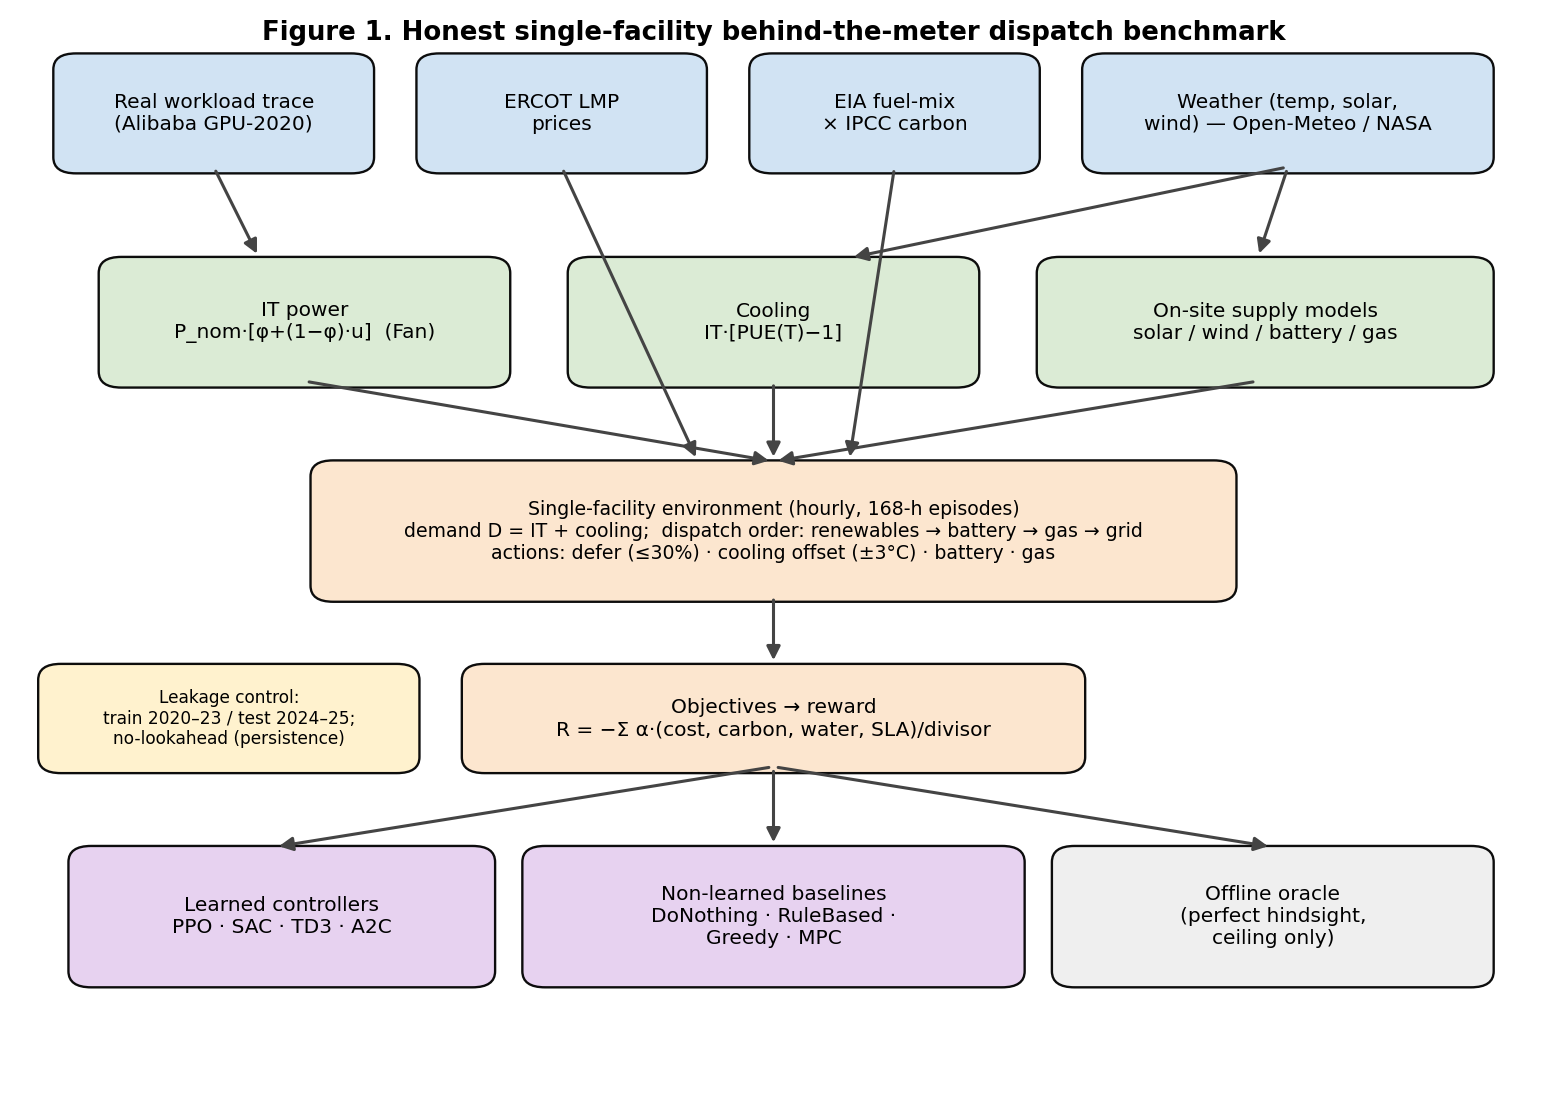
\includegraphics[keepaspectratio,alt={Figure 1}]{figures/fig1_system_schematic.png}}
\emph{Figure 1. The benchmark pipeline: real data inputs (workload
trace, ERCOT prices, EIA-derived carbon, weather) drive the substrate
models (Fan IT-power, PUE(T) cooling, on-site supply) and the
single-facility environment (dispatch order
renewables→battery→gas→grid); the weighted objective is optimized by the
learned and non-learned controllers and bounded by the offline LP
optimum, all under the leakage-control protocol (2020--23 train /
2024--25 test, no-lookahead forecast).}

\subsubsection{3.1 Facility and assets}\label{facility-and-assets}

A single data center with IT nameplate P\_nom = 20 MW and idle fraction
φ = 0.30. On-site assets at design sizing: 5 MW solar, 5 MW wind, a 20
MWh battery rated at 10 MW (C/2) with a \textbf{0.90 round-trip
efficiency} (√0.90 ≈ 0.949 applied at each of charge and discharge;
§3.4), and a 2 MW gas generator with a CO₂ emission factor of 0.41
kgCO₂/kWh (EIA/EPA natural-gas electricity, \textasciitilde0.91 lb
CO₂/kWh). We study the \textbf{twelve} source configurations obtained by
enabling subsets of \{solar, wind, battery, gas\} on top of the
always-present grid tie (grid\_only, grid\_solar, grid\_wind, grid\_gas,
grid\_solar\_wind, grid\_solar\_battery, grid\_wind\_battery,
grid\_solar\_gas, grid\_wind\_gas, grid\_solar\_wind\_battery,
grid\_solar\_wind\_gas, all\_sources). This factorial design attributes
any controller advantage to specific asset types rather than the
aggregate.

\subsubsection{3.2 Real workload trace → IT
power}\label{real-workload-trace-it-power}

IT load is driven by a \textbf{replayed real workload trace}, not a
synthetic profile. From the Alibaba \texttt{cluster-trace-gpu-v2020}
trace we reconstruct hourly cluster utilization by replaying instance
start/end events weighted by per-instance usage and normalizing by
machine capacity (the method established for this trace, Weng et
al.~2022). Because the trace timestamps are desensitized (time-of-day
and day-of-week are real, calendar dates are not), we collapse the
reconstruction into a \textbf{typical-week profile} of 168 values
indexed by (day-of-week × 24 + hour-of-day) and replay it onto the
2020--2025 timestamp axis. Utilization u(t) ∈ {[}0,1{]} maps to IT power
through a linear idle/peak envelope (Fan et al.~2007):

IT(t) = P\_nom · {[} φ + (1 − φ) · u(t) {]}, with P\_nom = 20 MW, φ =
0.30.

The reconstructed load is diurnally structured but relatively flat: the
replayed typical-week profile the agent actually sees has mean ≈ 12\%
and peak ≈ 15\% of capacity (the raw pre-aggregation hourly trace peaks
at ≈ 25\%, smoothed by the typical-week averaging) --- a genuine
property of ML clusters, disclosed as a limit on deferral headroom (§7).

\pandocbounded{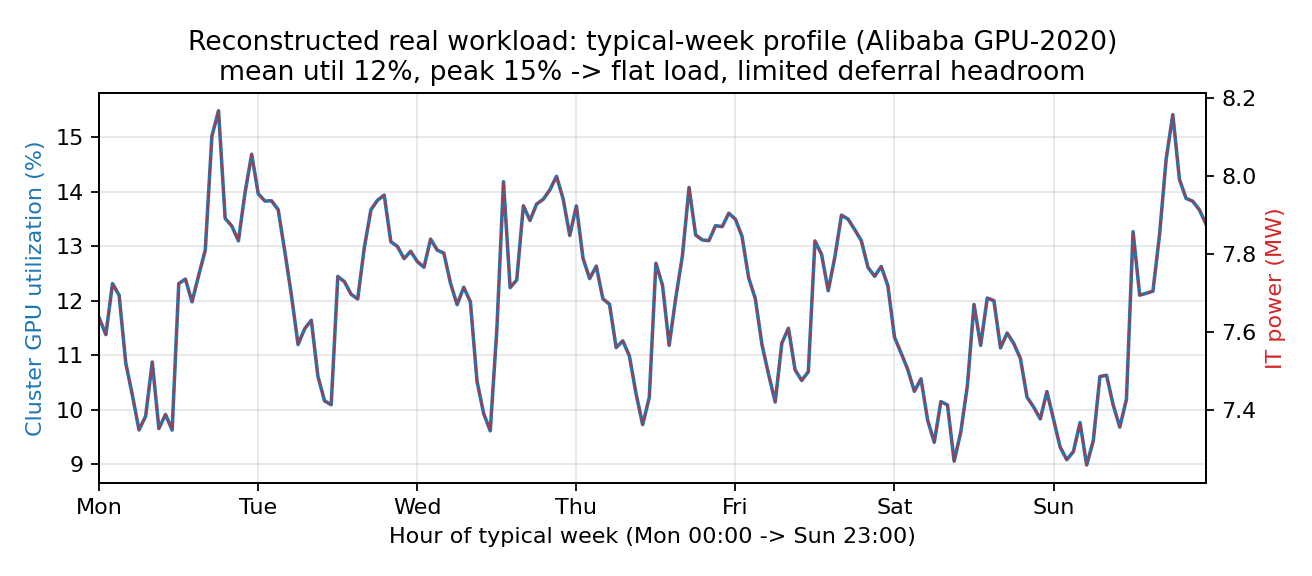
\includegraphics[keepaspectratio,alt={Figure 2}]{figures/fig_load_typical_week.png}}
\emph{Figure 2. Reconstructed typical-week workload (Alibaba GPU-2020):
cluster GPU utilization and the derived IT power. The load is diurnal
but relatively flat, limiting deferral headroom.}

\subsubsection{3.3 Physical cooling}\label{physical-cooling}

Cooling power is derived from IT power and real ambient temperature T(t)
via a temperature-dependent PUE:

cooling(t) = IT(t) · {[} PUE(T(t)) − 1 {]}, PUE(T) = PUE\_min + s ·
max(0, T − T\_ref), PUE\_min = 1.25, s = 0.01 /°C, T\_ref = 20 °C.

The uncontrolled facility demand is D(t) = IT(t) + cooling(t) (mean ≈
9.7 MW at design sizing).

\subsubsection{3.4 On-site generation and storage
models}\label{on-site-generation-and-storage-models}

\emph{Solar (5 MW):} from shortwave irradiance G(t) (W/m²), P\_solar(t)
= clip( G(t) · 32,679 · 0.18 · 0.85 / 1000, 0, 5000 ) kW --- i.e.~a
32,679 m² array at 18\% module efficiency and 0.85 performance ratio,
sized to reach the 5 MW nameplate at 1000 W/m². The array is driven by
the data center's own ambient weather, giving a \textasciitilde17\%
capacity factor --- lower than a purpose-sited utility solar farm --- so
solar-config savings here are conservative. \emph{Wind (5 MW):} a cubic
power curve in wind speed v(t) (m/s) with cut-in 3.5, rated 12, cut-out
25: P\_wind = 5000 · ((v − 3.5)/8.5)³ for 3.5 ≤ v \textless{} 12; 5000
for 12 ≤ v ≤ 25; 0 otherwise. \emph{Battery:} SoC-tracked with a
\textbf{0.90 round-trip efficiency} (√0.90 ≈ 0.949 applied at each of
charge and discharge, so the product is 0.90) and a power cap of 10 MW;
grid charging incurs cost and carbon at the current LMP/intensity, while
excess renewable (generation above demand) charges the battery for free
up to 95\% SoC. This free renewable charging is applied automatically
\textbf{regardless of the agent's battery action} --- surplus on-site
generation is never spilled while headroom exists --- so the SoC
transition is not fully determined by the agent's explicit battery
command. All inputs to this rule (SoC, current renewable availability,
demand) are in the observation, so the dynamic is Markov-preserving; it
reduces the agent's direct control authority over SoC without hiding
state (revisited in §7 Threat \#11 and §6.2 as one reason storage
coordination is hard). \emph{Gas:} dispatchable up to 2 MW at Henry Hub
cost and 0.41 kgCO₂/kWh (§3.1).

\subsubsection{3.5 Real market and environmental
data}\label{real-market-and-environmental-data}

Dispatch runs on real ERCOT LMPs; grid carbon intensity is the EIA
hourly fuel mix combined with IPCC emission factors; weather
(temperature, humidity, solar irradiance, wind speed) is measured
(Open-Meteo / NASA POWER). CAISO price history begins only in 2023 and
is excluded from the multi-year run to keep the market signal consistent
across the full 2020--2025 span (§7).

\subsubsection{3.6 State, actions, and load
dynamics}\label{state-actions-and-load-dynamics}

The \textbf{observation} is an 18-dimensional vector of normalized
signals: cyclical hour and month encodings; normalized IT load, cooling
load, temperature, humidity, solar irradiance, and wind speed;
normalized grid price, grid carbon, and gas price; battery SoC;
normalized available solar and wind; and two price-forecast inputs at 4
h and 24 h (see §4.1). The \textbf{action} is four continuous controls:
workload deferral a₁ ∈ {[}0,1{]} (scaled to a hard cap of 30\% of load),
cooling setpoint offset a₂ ∈ {[}−1,1{]} (mapped to ±3 °C, which scales
mechanical cooling by 1 − 0.03·offset and evaporative water by 1 +
0.05·offset), battery signal a₃ ∈ {[}−1,1{]} (negative = charge,
positive = discharge), and gas dispatch fraction a₄ ∈ {[}0,1{]}.
Deferred work accumulates up to a ceiling of 30\% × load × 12 h; when
the ceiling is exceeded the excess is force-served and an \textbf{SLA
violation} is recorded, and one-twelfth of the deferred backlog is
served each hour. Served demand is met in the priority order
\textbf{renewables → battery → gas → grid}, so zero-marginal-cost
on-site generation is always used first.

\subsubsection{3.7 Objectives and reward}\label{objectives-and-reward}

Per hour we accumulate three physical costs from the dispatch above:
monetary cost (battery grid-charging + gas + grid draw, each × its
price), carbon (same energies × their carbon factors), and water via an
evaporative model water(t) = cooling(t) · 1.8 · h\_f · T\_f · w\_f /
1000 {[}m³{]}, where h\_f = 1 + (50 − RH)/100 (drier air evaporates more
water per unit of cooling); the 1.8 base coefficient is a mid-range
water-usage-effectiveness value for evaporative data-center cooling and
enters only the water objective (its sensitivity scope is in Table VI).
Here T\_f = 1.2 if T \textgreater{} 25 °C, 0.5 if T \textless{} 10 °C,
else 1.0, and w\_f = 1 + 0.05·offset. The reward is the negative
weighted sum of the four \textbf{normalized} objectives:

R(t) = − ( α\_cost · cost/C + α\_carbon · carbon/K + α\_water · water/W
+ α\_sla · SLA ),

where SLA is a \textbf{latching} penalty: once any violation has
occurred in the episode, the full α\_sla term is charged every remaining
hour (so a single early violation can incur up to \textasciitilde167
penalty-hours), which makes the SLA term a strong deterrent against ever
exceeding the deferral ceiling. The divisors C, K, W are the mean hourly
cost, carbon, and water over the loaded substrate --- computed
\textbf{from the data}, not hand-set: C = mean(D·price) = 592.1, K =
mean(D·carbon) = 3683.7, W = mean(water\_ref) = 2.638. Data-derived
divisors keep every objective at order ≈ 1 so none silently dominates,
and they recalibrate automatically if the substrate changes. The
divisors depend only on the loaded substrate, and every reported verdict
compares controllers \emph{within the same configuration} (RL against
the baselines on identical divisors, weights, and weeks), so the
normalization sets the scale of the training reward but cannot bias the
RL-vs-heuristic comparison. Unless a sweep overrides them (§5.7), the
weights are α = (cost 0.4, carbon 0.3, water 0.2, SLA 0.1).

\subsubsection{3.8 Parameter summary}\label{parameter-summary}

Table V consolidates the substrate and control parameters for
reproducibility; all are fixed across configurations and seeds (asset
capacities are zeroed when a source is disabled).

\textbf{TABLE V --- Substrate and control parameters.}

{\def\LTcaptype{none} % do not increment counter
\begin{longtable}[]{@{}
  >{\raggedright\arraybackslash}p{(\linewidth - 4\tabcolsep) * \real{0.3333}}
  >{\raggedright\arraybackslash}p{(\linewidth - 4\tabcolsep) * \real{0.3333}}
  >{\raggedright\arraybackslash}p{(\linewidth - 4\tabcolsep) * \real{0.3333}}@{}}
\toprule\noalign{}
\begin{minipage}[b]{\linewidth}\raggedright
Group
\end{minipage} & \begin{minipage}[b]{\linewidth}\raggedright
Parameter
\end{minipage} & \begin{minipage}[b]{\linewidth}\raggedright
Value
\end{minipage} \\
\midrule\noalign{}
\endhead
\bottomrule\noalign{}
\endlastfoot
IT power & nameplate P\_nom; idle fraction φ & 20 MW; 0.30 \\
Cooling & PUE\_min; slope s; T\_ref & 1.25; 0.01 /°C; 20 °C \\
Solar & nameplate; area; module eff.; perf. ratio & 5 MW; 32,679 m²;
0.18; 0.85 \\
Wind & nameplate; cut-in / rated / cut-out & 5 MW; 3.5 / 12 / 25 m/s \\
Battery & capacity; power cap; round-trip η (√0.90 each end);
free-charge SoC cap & 20 MWh; 10 MW; 0.90; 0.95 \\
Gas & capacity; emission factor & 2 MW; 0.41 kgCO₂/kWh (EIA/EPA) \\
Deferral / SLA & max per-hour deferral; accumulation ceiling & 30\% of
load; 30\%·load·12 h \\
Cooling action & setpoint offset; mech. scale; water scale & ±3 °C; 1 −
0.03·offset; 1 + 0.05·offset \\
Water model & base coeff.; humidity factor; temp factor & 1.8; 1 +
(50−RH)/100; 1.2 / 1.0 / 0.5 \\
Reward weights & α (cost / carbon / water / SLA) & 0.4 / 0.3 / 0.2 /
0.1 \\
Reward divisors & C / K / W (data-derived) & 592.1 / 3683.7 / 2.638 \\
Episode / split & length; train / test; test indices & 168 h; 2020--23 /
2024--25; {[}35064, 52272{]} \\
Evaluation & held-out episodes; matched seeds & 200; 8000--8199 \\
Training & steps/run; parallel envs; total campaign & 1×10⁶; 4; 445 runs
(240 main + 120 foresight PPO+SAC + 80 Pareto @20 seeds + 5 sizing) \\
\end{longtable}
}

\begin{center}\rule{0.5\linewidth}{0.5pt}\end{center}

\subsection{4. EXPERIMENTAL DESIGN}\label{experimental-design}

\subsubsection{4.1 Leakage controls}\label{leakage-controls}

Two mechanisms enforce honesty and are the methodological core of the
paper.

\emph{Temporal split.} Training episodes are restricted to start indices
whose entire one-week horizon lies before the split date of 1 January
2024; evaluation episodes are drawn only from the held-out 2024--2025
period (environment step indices {[}35064, 52272{]}). Nothing an agent
sees at test time was available during training.

\emph{No lookahead.} The environment exposes a forecast mode. In the
reported condition, \texttt{persistence}, the controller's 4-hour and
24-hour price-forecast inputs are simply the current price, so the agent
receives no future information. A second mode, \texttt{oracle}, injects
the true future price and is used \textbf{only} for the labeled
foresight ablation in §5.6; it is never a headline result.

\subsubsection{4.2 Baselines (exact
definitions)}\label{baselines-exact-definitions}

All baselines act on the same 18-dim observation and 4-dim action space
as the RL agents, so the comparison is like-for-like. We define them
precisely for reproducibility.

\begin{itemize}
\tightlist
\item
  \textbf{DoNothing} --- action (0, 0, 0, 0): no deferral, no cooling
  offset, no battery or gas dispatch. Renewables are still consumed
  automatically (they sit first in the dispatch order), so this is the
  ``grid + free renewables'' floor.
\item
  \textbf{RuleBased} (time-of-use heuristic, the headline comparator)
  --- fixed deferral a₁ = 0.6 (≈18\% of load); battery charge a₃ = −0.7
  during 01:00--05:00 and discharge a₃ = +0.8 during 16:00--21:00, else
  idle; gas a₄ = 0.8 during 16:00--20:00, else 0; no cooling offset.
\item
  \textbf{Greedy} (myopic price response, no foresight) --- defer a₁ =
  0.8 when the normalized price exceeds 0.3 else 0.2; discharge (a₃ =
  +0.6) when price is high, charge (a₃ = −0.6) when low, else idle;
  dispatch gas when it is cheaper than the grid.
\item
  \textbf{MPC} (forecast-driven control) --- compares the current price
  to its 4 h and 24 h forecast inputs, discharging/deferring when now
  looks expensive relative to the future and charging/running when it
  looks cheap. Under the reported \texttt{persistence} forecast these
  inputs equal the current price, so its look-ahead signal is ≈0 and it
  degrades toward inaction --- a \emph{naive-forecast} MPC, stated
  explicitly and revisited in §5.5.
\item
  \textbf{LP optimum} (offline economic-dispatch ceiling, perfect
  foresight) --- for each episode we solve a linear program that
  minimizes total dispatch cost (grid draw + gas + grid-charging)
  subject to the exact physical constraints every controller faces:
  battery state-of-charge dynamics with the 0.90 round-trip efficiency
  and 10 MW power cap, 0 ≤ SoC ≤ capacity, gas capacity, hour-by-hour
  energy balance with renewables used first, and workload deferral
  modeled with the environment's own SLA-avoiding 1/12-per-hour backlog
  drain. Solved with perfect price/renewable/demand foresight (HiGHS),
  it is a genuine per-episode cost minimum --- a per-episode lower bound
  on achievable dispatch cost, verified to satisfy LP ≤ RuleBased on
  every episode. It replaces the quantile-threshold rule (charge in the
  cheapest price quartile, discharge in the most expensive) that much of
  this literature labels the ``oracle''; that rule ignores SoC and
  coupling and is itself far from optimal, so it \emph{understates} the
  optimality gap (§5.2). The LP is deliberately conservative in one
  respect --- it does not exploit the cooling-offset cost lever --- so
  its reported gap is a lower bound on the unrestricted one. Because it
  fixes the cooling lever and assumes perfect foresight, we call it the
  \textbf{offline (cost-optimal dispatch) optimum}: a tight
  \emph{offline} benchmark for the dispatch of
  battery/gas/grid/deferral, not a claim of global optimality over every
  control lever. It is a ceiling for measurement, never a deployable
  controller. The LP minimizes \textbf{cost only}, whereas the RL reward
  is multi-objective; we compare on \textbf{cost} because cost carries
  the dominant weight (α = 0.4) and is the reported metric, and because
  this makes the comparison \emph{conservative} toward RL --- a
  cost-only optimum is the easiest target for a cost-bearing controller
  to approach, so the gap we attribute to a learner is if anything
  understated by its attention to carbon/water. The cost-heavy Pareto
  point (§5.7), where RL is re-weighted almost entirely toward cost and
  still leaves the storage gap open, confirms the gap is not an artifact
  of this multi-objective asymmetry.
\end{itemize}

\subsubsection{4.3 Learned controllers}\label{learned-controllers}

We train \textbf{PPO} (Schulman et al.~2017), \textbf{SAC} (Haarnoja et
al.~2018), \textbf{TD3} (Fujimoto et al.~2018), and \textbf{A2C} (Mnih
et al.~2016), all via Stable-Baselines3 (Raffin et al.~2021), with a
shared MLP policy and identical hyperparameters across all
configurations, so differences reflect the configuration and the
algorithm, not per-case tuning. The shared-hyperparameter design is
deliberate: per-configuration tuning would introduce exactly the
optimistic bias (tuning on the evaluation distribution) that inflates RL
results in this literature, so we forgo it and report the untuned
learners. Salient settings: learning rate 3×10⁻⁴ (7×10⁻⁴ for A2C), γ =
0.99, GAE λ = 0.95; PPO with n\_steps 2048, batch 64, 10 epochs, clip
0.2; SAC/TD3 with replay buffer 10⁵ and batch 256 (SAC with automatic
entropy tuning); A2C at the Stable-Baselines3 default n\_steps = 5. Each
run trains for 1×10⁶ steps with four parallel environments. One caveat
follows from using stock per-algorithm defaults: A2C's 5-step rollout is
short for the 168-hour storage credit-assignment problem (a charge
decision often pays off many hours later), so A2C's comparatively large
storage losses (§5.4) partly reflect this hyperparameter mismatch rather
than a pure algorithmic property. We report A2C as-is for completeness
but base the headline verdict on the best-of-four algorithm per
configuration. All four use \textbf{feedforward (MLP) policies};
recurrent policies (LSTM/Transformer), which are the natural
architecture for long-horizon storage credit assignment, are out of
scope here and are the most important learned-control extension we flag
for future work (§6.6). The storage findings below should therefore be
read as a result about \emph{memoryless} learned controllers under this
training budget.

\subsubsection{4.4 Protocol and
statistics}\label{protocol-and-statistics}

We train \textbf{240 policies} (4 algorithms × 12 configurations × 5
seeds) with hardened checkpointing: a held-out evaluation is logged at
every 100k-step checkpoint, and for the off-policy methods the replay
buffer is persisted so a resumed run does not silently train on a
degraded buffer. Every controller --- RL and baseline alike --- is
evaluated on \textbf{200 held-out episodes with matched seeds
8000--8199}, so all methods are scored on identical weeks. We compare
per-episode cost with paired tests and \textbf{Holm-correct across the
full family of 48 tests (4 algorithms × 12 configurations)}, and report
Wilcoxon signed-rank tests, bootstrap 95\% confidence intervals, and
Cohen's d alongside. A result is ``significant'' only when the
Holm-adjusted p \textless{} 0.05 \textbf{and} the direction favors the
named controller. Two properties of the comparison should be read
alongside these statistics. First, the RL cost fed into each paired test
is the \textbf{per-episode mean across the five seeds} (a five-policy
ensemble), whereas each baseline is a single deterministic run;
averaging shrinks the RL per-episode variance by roughly √5, which
raises the paired test's power asymmetrically and matters most at the
smallest (0.5--1.1\%) renewable-only margins. Second, because every
controller is scored on the \emph{same} price/weather weeks, per-episode
costs are highly correlated and the paired-difference standard deviation
is small, so Cohen's d is inflated relative to the economic effect (e.g.
d ≈ 0.84 accompanies a 0.51\% cost change); we therefore treat the
\textbf{bootstrap 95\% CI on the mean cost difference} as the primary
effect-size and read d only as a secondary signal. To avoid a
garden-of-forking-paths, the substrate and hyperparameters were fixed
before the held-out evaluation and not tuned against it; the real
workload and sizing sweeps are pre-registered robustness checks reported
either way.

\begin{center}\rule{0.5\linewidth}{0.5pt}\end{center}

\subsection{5. RESULTS}\label{results}

\subsubsection{5.1 A note on the comparison
baseline}\label{a-note-on-the-comparison-baseline}

The headline comparator is the RuleBased heuristic. Table I shows why:
across the full matched-protocol baseline set, RuleBased is the
lowest-cost non-oracle controller in every configuration except the four
gas configurations, where Greedy edges it by less than 0.1\%. It is, in
other words, the strongest cheap controller, and the fair opponent for a
learned policy.

\textbf{TABLE I --- Matched-protocol weekly cost (USD), held-out test, n
= 200, persistence forecast. Lowest-cost controller in bold; ``MPC−RB''
is MPC's penalty relative to RuleBased. The ``MPC'' column is a
\emph{naive-forecast} MPC: under the persistence forecast its look-ahead
signal is ≈0, so it degrades toward inaction (§5.5) --- it is not a
competent forecast-driven controller.}

{\def\LTcaptype{none} % do not increment counter
\begin{longtable}[]{@{}
  >{\raggedright\arraybackslash}p{(\linewidth - 10\tabcolsep) * \real{0.1304}}
  >{\raggedleft\arraybackslash}p{(\linewidth - 10\tabcolsep) * \real{0.1739}}
  >{\raggedleft\arraybackslash}p{(\linewidth - 10\tabcolsep) * \real{0.1739}}
  >{\raggedleft\arraybackslash}p{(\linewidth - 10\tabcolsep) * \real{0.1739}}
  >{\raggedleft\arraybackslash}p{(\linewidth - 10\tabcolsep) * \real{0.1739}}
  >{\raggedleft\arraybackslash}p{(\linewidth - 10\tabcolsep) * \real{0.1739}}@{}}
\toprule\noalign{}
\begin{minipage}[b]{\linewidth}\raggedright
Configuration
\end{minipage} & \begin{minipage}[b]{\linewidth}\raggedleft
DoNothing
\end{minipage} & \begin{minipage}[b]{\linewidth}\raggedleft
RuleBased
\end{minipage} & \begin{minipage}[b]{\linewidth}\raggedleft
Greedy
\end{minipage} & \begin{minipage}[b]{\linewidth}\raggedleft
MPC
\end{minipage} & \begin{minipage}[b]{\linewidth}\raggedleft
MPC−RB
\end{minipage} \\
\midrule\noalign{}
\endhead
\bottomrule\noalign{}
\endlastfoot
grid\_only & 50,747 & \textbf{50,095} & 50,263 & 50,312 & +0.4\% \\
grid\_solar & 46,114 & \textbf{45,462} & 45,630 & 45,679 & +0.5\% \\
grid\_wind & 38,545 & \textbf{37,893} & 38,061 & 38,110 & +0.6\% \\
grid\_solar\_wind & 33,912 & \textbf{33,263} & 33,429 & 33,478 &
+0.6\% \\
grid\_gas & 50,747 & 48,550 & \textbf{48,531} & 50,018 & +3.0\% \\
grid\_solar\_gas & 46,114 & 43,916 & \textbf{43,898} & 45,385 &
+3.3\% \\
grid\_wind\_gas & 38,545 & 36,348 & \textbf{36,329} & 37,816 & +4.0\% \\
grid\_solar\_wind\_gas & 33,912 & 31,719 & \textbf{31,711} & 33,184 &
+4.6\% \\
grid\_solar\_battery & 46,114 & \textbf{42,919} & 44,967 & 45,679 &
+6.4\% \\
grid\_wind\_battery & 38,545 & \textbf{35,041} & 37,396 & 38,110 &
+8.8\% \\
grid\_solar\_wind\_battery & 33,912 & \textbf{29,834} & 32,729 & 33,478
& +12.2\% \\
all\_sources & 33,912 & \textbf{28,998} & 31,103 & 33,184 & +14.4\% \\
\end{longtable}
}

\subsubsection{\texorpdfstring{5.2 How far is the heuristic from the
\emph{offline} optimum? Not near, where it
counts.}{5.2 How far is the heuristic from the offline optimum? Not near, where it counts.}}\label{how-far-is-the-heuristic-from-the-offline-optimum-not-near-where-it-counts.}

A central methodological choice is the ceiling. Much of this literature
calls a quantile-threshold rule (charge in the cheapest price quartile,
discharge in the most expensive) the ``oracle.'' That rule ignores
state-of-charge limits and inter-hour coupling, so it is itself far from
optimal, and comparing against it manufactures a flattering conclusion.
Measured against it, RuleBased looks ``near-optimal'': the
RB→quantile-oracle gap is only 4--7\% for storage configs and even
\emph{touches zero} at a 40 MWh battery (Table IV, right block).
Measured against the \textbf{offline LP optimum}, the picture inverts.

Table Ib reports, per configuration, how far RuleBased and the best RL
controller sit above the genuine per-episode LP optimum (§4.2). The
heuristic is near-optimal \emph{only} in renewable-only dispatch
(6.0--9.0\%); in every storage-rich configuration it leaves
\textbf{20--25\%} on the table, and RL is further still. The quantile
oracle understated this gap by 3--5×.

\textbf{TABLE Ib --- Distance above the OFFLINE LP optimum (held-out
test, n = 200). Gap = (cost − LP)/cost. ``Quantile-oracle gap'' is the
old, weak ceiling shown for contrast. LP ≤ RuleBased every config.}

{\def\LTcaptype{none} % do not increment counter
\begin{longtable}[]{@{}
  >{\raggedright\arraybackslash}p{(\linewidth - 12\tabcolsep) * \real{0.1111}}
  >{\raggedleft\arraybackslash}p{(\linewidth - 12\tabcolsep) * \real{0.1481}}
  >{\raggedleft\arraybackslash}p{(\linewidth - 12\tabcolsep) * \real{0.1481}}
  >{\raggedleft\arraybackslash}p{(\linewidth - 12\tabcolsep) * \real{0.1481}}
  >{\raggedleft\arraybackslash}p{(\linewidth - 12\tabcolsep) * \real{0.1481}}
  >{\raggedleft\arraybackslash}p{(\linewidth - 12\tabcolsep) * \real{0.1481}}
  >{\raggedleft\arraybackslash}p{(\linewidth - 12\tabcolsep) * \real{0.1481}}@{}}
\toprule\noalign{}
\begin{minipage}[b]{\linewidth}\raggedright
Configuration
\end{minipage} & \begin{minipage}[b]{\linewidth}\raggedleft
RuleBased \$
\end{minipage} & \begin{minipage}[b]{\linewidth}\raggedleft
Best RL \$
\end{minipage} & \begin{minipage}[b]{\linewidth}\raggedleft
LP optimum \$
\end{minipage} & \begin{minipage}[b]{\linewidth}\raggedleft
RB→opt
\end{minipage} & \begin{minipage}[b]{\linewidth}\raggedleft
RL→opt
\end{minipage} & \begin{minipage}[b]{\linewidth}\raggedleft
(old quantile-oracle RB gap)
\end{minipage} \\
\midrule\noalign{}
\endhead
\bottomrule\noalign{}
\endlastfoot
grid\_only & 50,095 & 49,869 & 47,091 & 6.0\% & 5.6\% & 3.0\% \\
grid\_solar & 45,462 & 44,958 & 42,457 & 6.6\% & 5.6\% & 3.3\% \\
grid\_wind & 37,893 & 37,617 & 34,889 & 7.9\% & 7.3\% & 3.9\% \\
grid\_solar\_wind & 33,263 & 32,736 & 30,265 & 9.0\% & 7.5\% & 4.5\% \\
grid\_gas & 48,550 & 48,926 & 43,844 & 9.7\% & 10.4\% & 4.9\% \\
grid\_solar\_gas & 43,916 & 44,041 & 39,210 & 10.7\% & 11.0\% & --- \\
grid\_wind\_gas & 36,348 & 36,258 & 31,642 & 12.9\% & 12.7\% & 6.6\% \\
grid\_solar\_wind\_gas & 31,719 & 31,586 & 27,112 & 14.5\% & 14.2\% &
--- \\
grid\_solar\_battery & 42,919 & 43,461 & 34,199 & \textbf{20.3\%} &
21.3\% & 4.8\% \\
grid\_wind\_battery & 35,041 & 35,979 & 27,603 & \textbf{21.2\%} &
23.3\% & 4.4\% \\
grid\_solar\_wind\_battery & 29,834 & 30,734 & 23,349 & \textbf{21.7\%}
& 24.0\% & 4.7\% \\
all\_sources & 28,998 & 30,450 & 21,725 & \textbf{25.1\%} & 28.7\% &
6.9\% \\
\end{longtable}
}

So the well-worn ``heuristic is near-optimal'' claim is an artifact of a
weak oracle. Against a real optimum, both a well-tuned heuristic and RL
leave \textbf{\textasciitilde a fifth to a quarter of the storage bill
unclaimed} --- a large online-to-offline gap that neither controller
here closes, and that RL actually \emph{widens}. Renewable-only dispatch
is the only regime where the heuristic genuinely comes close (6--9\%).
This gap --- not a 1\% RL-vs-heuristic delta --- is the central finding.

\pandocbounded{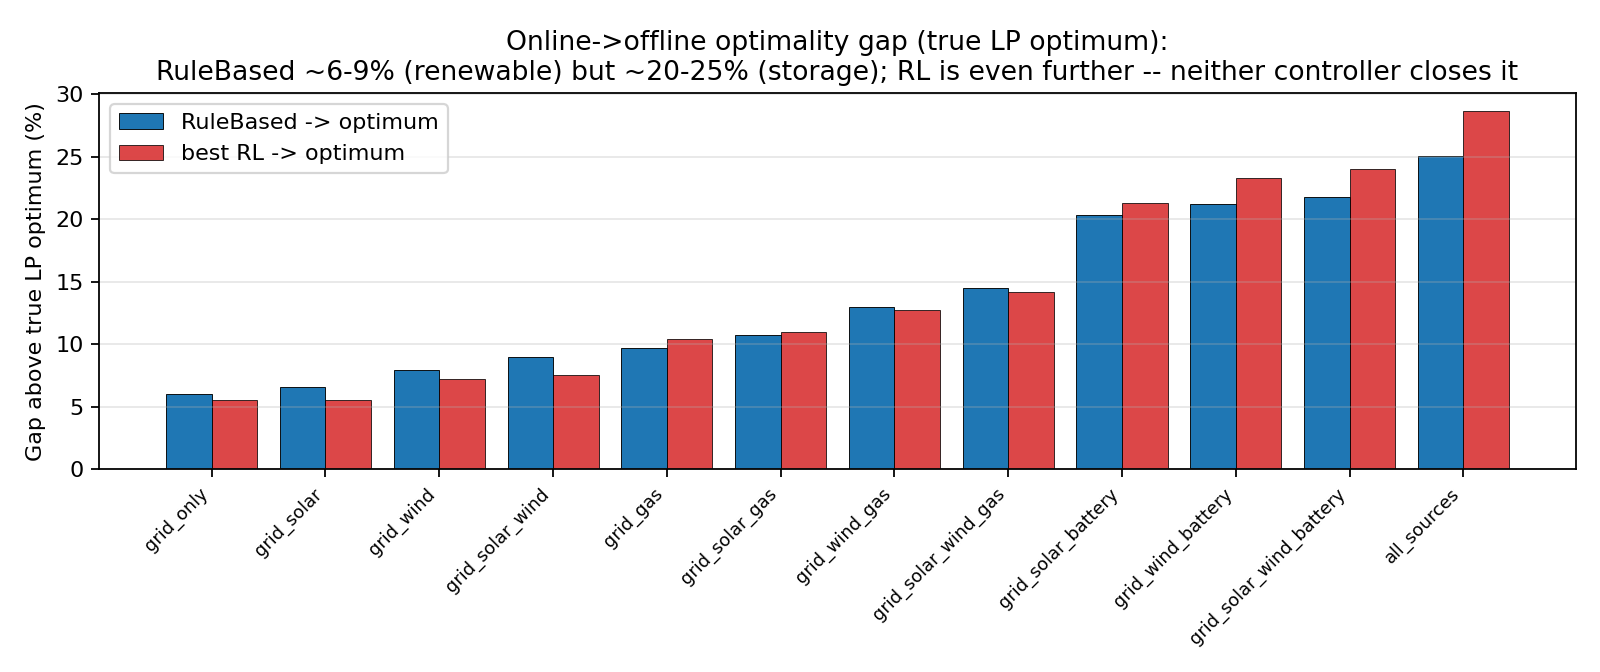
\includegraphics[keepaspectratio,alt={Figure 3}]{figures/fig_optimality_gap.png}}
\emph{Figure 3. Distance above the offline LP optimum, per
configuration. RuleBased (blue) is within \textasciitilde6--9\% in
renewable-only dispatch but \textasciitilde20--25\% above optimum in
storage-rich configs; the best RL controller (red) is further still.
Neither closes the online-to-offline gap.}

\subsubsection{5.3 Main benchmark: does RL beat the
heuristic?}\label{main-benchmark-does-rl-beat-the-heuristic}

Table II reports, for each configuration, the best of the four RL
algorithms, its improvement over RuleBased, and whether that difference
is significant after Holm correction (across the 48-test family).

\textbf{TABLE II --- Best RL vs RuleBased on held-out cost (matched
seeds, n = 200). Positive Δ\% = cheaper than RuleBased. ``sig. loss'' =
the RL deficit is Holm-significant.}

{\def\LTcaptype{none} % do not increment counter
\begin{longtable}[]{@{}lrlrc@{}}
\toprule\noalign{}
Configuration & RuleBased & Best RL (algo) & Δ\% vs RB & Significant? \\
\midrule\noalign{}
\endhead
\bottomrule\noalign{}
\endlastfoot
grid\_only & 50,095 & 49,869 (SAC) & +0.45 & win \\
grid\_solar & 45,462 & 44,958 (SAC) & +1.11 & win \\
grid\_wind & 37,893 & 37,617 (SAC) & +0.73 & win \\
grid\_solar\_wind & 33,263 & 32,736 (TD3) & +1.58 & win \\
grid\_gas & 48,550 & 48,926 (PPO) & −0.78 & sig. loss \\
grid\_solar\_gas & 43,916 & 44,041 (PPO) & −0.28 & sig. loss \\
grid\_wind\_gas & 36,348 & 36,258 (SAC) & +0.25 & no \\
grid\_solar\_wind\_gas & 31,719 & 31,586 (TD3) & +0.42 & no \\
grid\_solar\_battery & 42,919 & 43,461 (PPO) & −1.26 & sig. loss \\
grid\_wind\_battery & 35,041 & 35,979 (PPO) & −2.68 & sig. loss \\
grid\_solar\_wind\_battery & 29,834 & 30,734 (PPO) & −3.02 & sig.
loss \\
all\_sources & 28,998 & 30,450 (PPO) & −5.01 & sig. loss \\
\end{longtable}
}

The best RL controller significantly beats RuleBased in \textbf{four of
twelve} configurations, and all four are renewable-only
(\texttt{grid\_only}, \texttt{grid\_solar}, \texttt{grid\_wind},
\texttt{grid\_solar\_wind}), with margins of 0.5--1.6\%. In the two
gas-only-adjacent wins (\texttt{grid\_wind\_gas},
\texttt{grid\_solar\_wind\_gas}) the best margin is +0.2--0.4\% and does
not clear Holm correction. Everywhere a battery is present --- and in
the two simplest gas configs --- RL is a \textbf{significant loss}. No
single algorithm dominates the wins (SAC and TD3 split them), which
argues against a robust learned advantage; PPO is uniformly the ``best''
(least-bad) algorithm in the storage configs, and even it loses.

\subsubsection{5.4 The storage-degradation
pattern}\label{the-storage-degradation-pattern}

The most consistent effect in the study is a failure, not a win. In
\textbf{every configuration that contains a battery}, the best RL
controller is \emph{worse} than the fixed RuleBased charge/discharge
schedule, and the loss deepens as the asset mix grows: −1.3\%
(\texttt{grid\_solar\_battery}), −2.7\% (\texttt{grid\_wind\_battery}),
−3.0\% (\texttt{grid\_solar\_wind\_battery}), and \textbf{−5.0\%}
(\texttt{all\_sources}) for the best algorithm in each case; the weaker
learners degrade further, and per-algorithm Holm tests confirm the
losses are significant. This is the opposite of the common assumption
that storage --- with its inter-temporal coupling --- is where learning
adds the most value.

Two readings are tempting; the offline-optimum ceiling (§5.2) forces the
correct one. It is \emph{not} that ``the fixed schedule is already
near-optimal, and RL merely mis-times against it'': against the LP
optimum the schedule itself leaves 20--25\% unclaimed on these very
configs (Table Ib). The accurate statement is that \textbf{storage makes
the problem hard for everyone, and hardest for the learner} --- a charge
decision pays off many hours later, so storage turns each hour into a
week-long credit-assignment problem that RL's value estimates handle
worst, leaving it \emph{below} even an imperfect fixed rule. The
degradation is not a sizing artifact: it persists across a fourfold
battery range (§5.8).

\pandocbounded{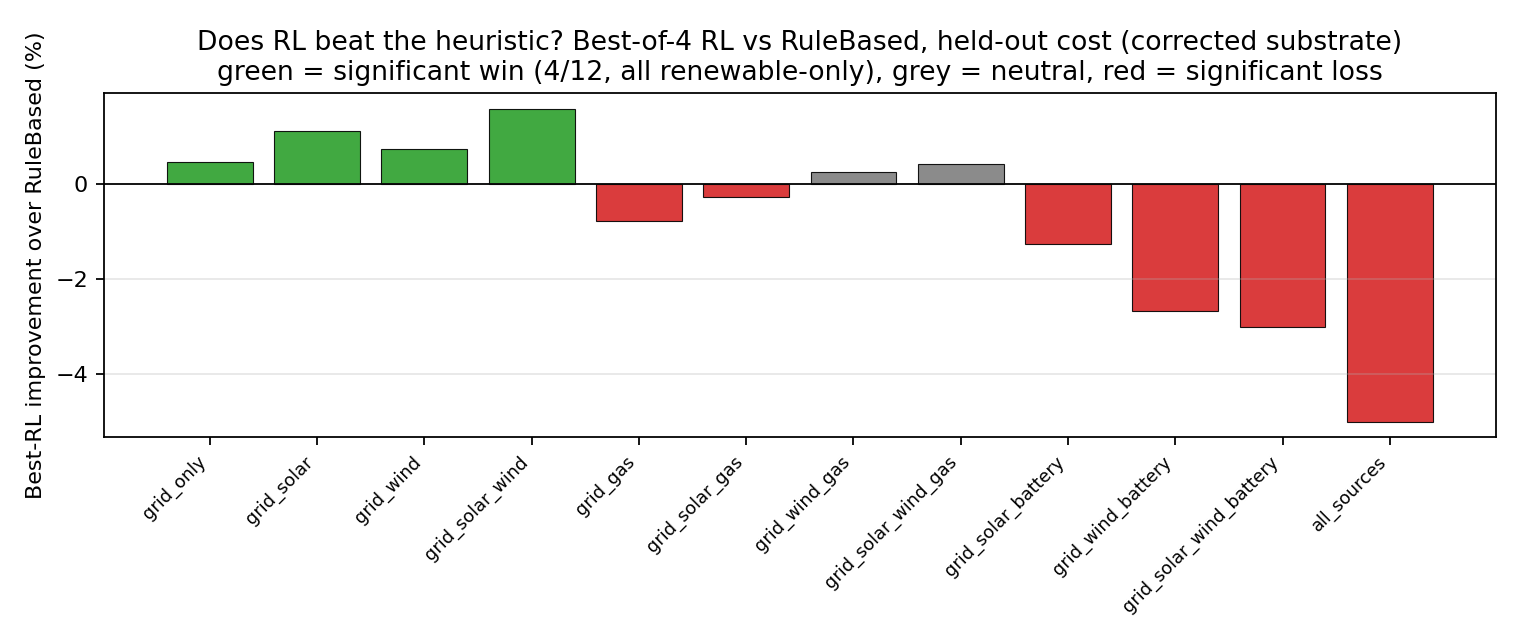
\includegraphics[keepaspectratio,alt={Figure 4}]{figures/fig_verdict_delta.png}}
\emph{Figure 4. Best-of-four RL improvement over RuleBased on held-out
cost, per configuration (green = significant win, grey = neutral, red =
significant loss). The four significant wins are all renewable-only
(0.5--1.6\%); every battery configuration is a significant loss,
deepening with asset-mix complexity to −5.0\% at the full mix.}

\subsubsection{5.5 The naive MPC, and where the real headroom
is}\label{the-naive-mpc-and-where-the-real-headroom-is}

Table I shows our MPC underperforming RuleBased everywhere, by +0.4\% in
the simplest cases and up to +14.4\% with the full asset mix. This is a
direct consequence of the honest protocol: with a persistence forecast,
MPC's price-versus-future signal is near zero, so its lookahead logic
rarely fires and it degrades toward a do-little controller. It is a
\emph{naive-forecast} MPC, not a competent one --- we include it only to
show that bolting a controller onto a zero-information forecast buys
nothing. We therefore read the MPC row as a \textbf{sanity floor, not as
evidence about the potential of competent forecast-driven control}, and
we do not draw any conclusion about MPC as a method from it. The fair
perfect-foresight reference point in this paper is the LP optimum; a
realistic-forecast MPC (finite forecast error, not zero information and
not perfect foresight) is the natural next controller and is deferred to
future work (§6).

The interesting question is what a \emph{good} forecast-driven optimizer
could do, and here the LP optimum is informative in a way the old
quantile ``oracle'' was not. The LP is precisely a perfect-foresight
receding-horizon optimizer solved to global optimality, and it captures
the 20--25\% storage headroom that RuleBased and RL both miss (§5.2). In
other words, the large online-to-offline gap is largely the \emph{value
of forecast-driven optimization that we did not attempt to realize
online}. This reframes forecast-MPC (e.g.~with a
Temporal-Fusion-Transformer price model, Lim et al.~2021) as the single
most promising direction for closing the gap. How much of the
perfect-foresight 20--25\% survives realistic forecast error is exactly
the open question this benchmark is built to pose; we leave the
forecast-MPC arm to future work and flag it as the natural next
controller, not a settled non-issue.

\subsubsection{5.6 Foresight-premium
ablation}\label{foresight-premium-ablation}

The common rebuttal to a weak RL showing is ``it would win with a better
forecaster.'' We test this directly by training \textbf{both PPO and
SAC} (the two algorithms that produce the wins and the least-bad storage
losses) across all twelve configurations with \textbf{perfect price
foresight} in the observation (\texttt{forecast\_mode\ =\ oracle}), and
comparing per-configuration held-out cost to the honest persistence
agents on identical seeds and window, with a per-episode paired test.
The \textbf{foresight premium} (persistence minus oracle cost) is
essentially zero for both: it averages \textbf{+0.08\% for PPO and
−0.37\% for SAC} (Table IIb; Figure 5). Where the premium is
statistically resolvable it is economically negligible (sub-1\% either
way), and SAC is if anything slightly \emph{worse} with foresight ---
consistent with overfitting a high-information input that does not
change the dispatch the agent can actually execute.

The force of this result comes from the contrast with §5.2:
\textbf{perfect foresight is worth 20--25\% to the LP optimum on storage
configs, but \textasciitilde0\% to the learned controllers.} Foresight
is not the missing ingredient for RL; the bottleneck is the agent's
inability to convert future information into correctly-timed multi-hour
storage decisions. The honest no-lookahead verdict therefore does not
understate RL --- its ceiling here is genuinely low, independent of
forecast quality --- even though the \emph{problem} has large foresight
value that a different (optimization-based) controller can capture.

\textbf{TABLE IIb --- Foresight premium (persistence minus oracle
cost)/persistence, per configuration, for PPO and SAC. Positive =
foresight makes the learner cheaper. Per-episode paired test.}

{\def\LTcaptype{none} % do not increment counter
\begin{longtable}[]{@{}lrr@{}}
\toprule\noalign{}
Configuration & PPO premium & SAC premium \\
\midrule\noalign{}
\endhead
\bottomrule\noalign{}
\endlastfoot
grid\_only & +0.24\% & +0.00\% \\
grid\_solar & −0.22\% & −0.01\% \\
grid\_wind & +0.49\% & +0.25\% \\
grid\_solar\_wind & +0.33\% & −0.24\% \\
grid\_gas & +0.24\% & +0.02\% \\
grid\_solar\_gas & −0.04\% & −0.05\% \\
grid\_wind\_gas & −0.92\% & −0.52\% \\
grid\_solar\_wind\_gas & +0.55\% & +0.16\% \\
grid\_solar\_battery & +0.10\% & +0.20\% \\
grid\_wind\_battery & −0.19\% & −3.00\% \\
grid\_solar\_wind\_battery & −1.07\% & −1.73\% \\
all\_sources & +1.39\% & +0.43\% \\
\end{longtable}
}

\emph{Mean premium: PPO +0.08\% (range −1.07..+1.39), SAC −0.37\% (range
−3.00..+0.43).}

\pandocbounded{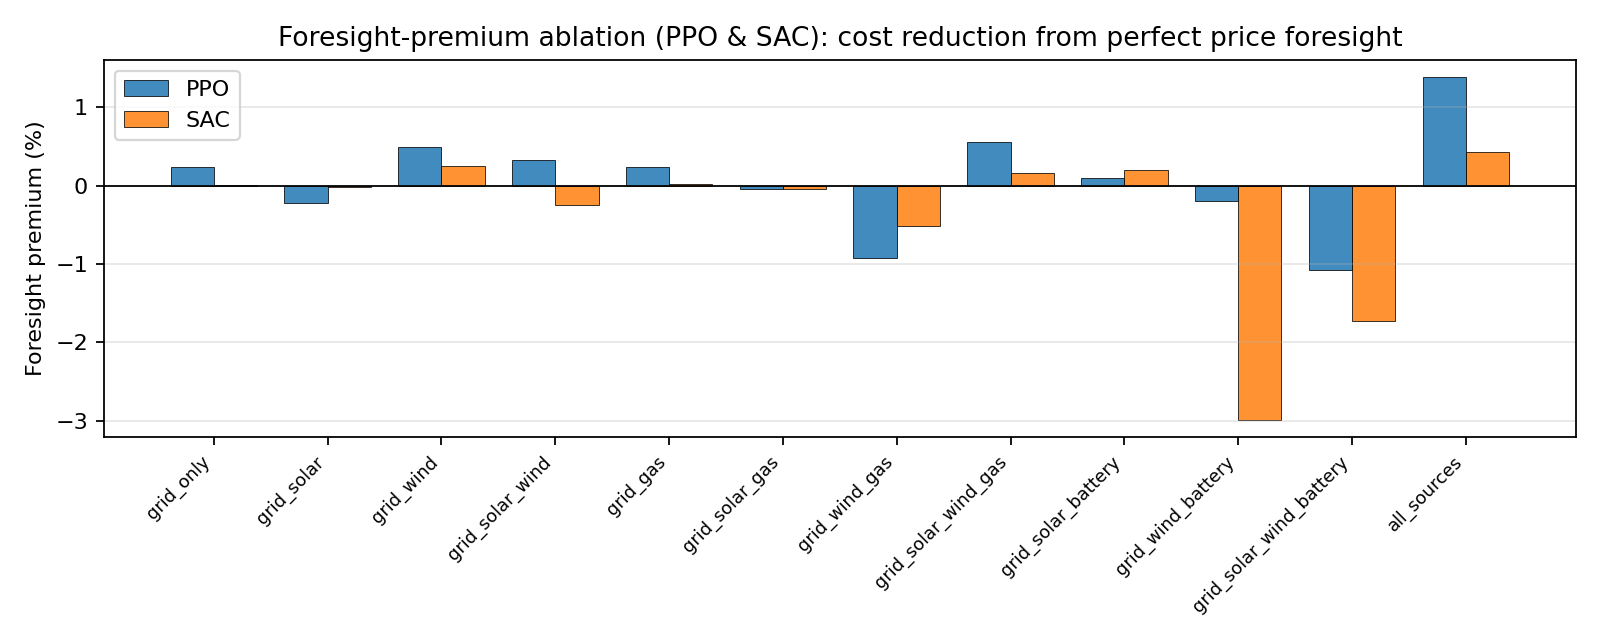
\includegraphics[keepaspectratio,alt={Figure 5}]{figures/fig_foresight_premium.png}}
\emph{Figure 5. Foresight premium per configuration for PPO and SAC ---
the held-out cost reduction from perfect price foresight. It hovers
around zero for both learners, even though the same perfect foresight is
worth 20--25\% to the LP optimum (§5.2): foresight is not the missing
ingredient for learned control in this regime.}

\subsubsection{5.7 Multi-objective weight
sweep}\label{multi-objective-weight-sweep}

Although RL does not beat the heuristic on the scalar objective, we ask
a distinct question: when RL \emph{is} used, do its reward weights give
an operator predictable control over the cost/carbon/water tradeoff? We
train PPO on \texttt{all\_sources} under four weightings --- cost-heavy,
carbon-heavy, water-heavy, and balanced --- with \textbf{20 seeds each}
(enough that the smaller levers are adequately powered), on the same
held-out window, with grid carbon as a \emph{visible} observation. This
is analyzed separately from the benchmark above, because the weighted
reward is not comparable across weightings.

\textbf{TABLE III --- Held-out weekly objectives by weighting (mean ±
95\% CI over 20 seeds); weights are cost/carbon/water/SLA.}

{\def\LTcaptype{none} % do not increment counter
\begin{longtable}[]{@{}
  >{\raggedright\arraybackslash}p{(\linewidth - 8\tabcolsep) * \real{0.1579}}
  >{\raggedleft\arraybackslash}p{(\linewidth - 8\tabcolsep) * \real{0.2105}}
  >{\raggedleft\arraybackslash}p{(\linewidth - 8\tabcolsep) * \real{0.2105}}
  >{\raggedleft\arraybackslash}p{(\linewidth - 8\tabcolsep) * \real{0.2105}}
  >{\raggedleft\arraybackslash}p{(\linewidth - 8\tabcolsep) * \real{0.2105}}@{}}
\toprule\noalign{}
\begin{minipage}[b]{\linewidth}\raggedright
Weighting
\end{minipage} & \begin{minipage}[b]{\linewidth}\raggedleft
Cost (USD)
\end{minipage} & \begin{minipage}[b]{\linewidth}\raggedleft
Carbon (kg CO₂)
\end{minipage} & \begin{minipage}[b]{\linewidth}\raggedleft
Water (m³)
\end{minipage} & \begin{minipage}[b]{\linewidth}\raggedleft
SLA (viol.)
\end{minipage} \\
\midrule\noalign{}
\endhead
\bottomrule\noalign{}
\endlastfoot
cost-heavy (0.7/0.1/0.1/0.1) & \textbf{29,396 ± 397} & 406,775 & 446.6 &
0.03 \\
carbon-heavy (0.1/0.7/0.1/0.1) & 31,829 & \textbf{400,157 ± 1,425} &
446.5 & 0.36 \\
water-heavy (0.1/0.1/0.7/0.1) & 32,705 & 409,336 & \textbf{437.4 ± 2.9}
& 0.00 \\
balanced (0.3/0.3/0.3/0.1) & 30,962 & 405,814 & 442.1 & 0.20 \\
\end{longtable}
}

The weighting knob behaves as designed: each single-objective-heavy
weighting minimizes its own objective (bold diagonal), all four points
are mutually Pareto-non-dominated, and --- with 20 seeds and grid carbon
among the observations --- all three levers are \textbf{statistically
significant}. The \emph{magnitudes}, however, separate a strong lever
from weak ones. Relative to the balanced point, the cost-heavy weighting
cuts cost by \textbf{5.1\%} (Welch p \textless{} 0.001), whereas the
carbon-heavy weighting cuts carbon by only \textbf{1.4\%} (p \textless{}
0.001) and the water-heavy weighting cuts water by \textbf{1.1\%} (p =
0.019). That the carbon/water effects are real but only
\textasciitilde1\% shows the weak carbon/water authority is
\textbf{physical, not an artifact}: renewables are already dispatched
first, the battery is grid-charged, and gas is carbon-dirty, so there is
little room to trade carbon or water without simply spending more. The
two aggressive weightings incur a small SLA cost (≈0.2--0.4
violations/week) versus near-zero for the water-heavy point. The
practical message: RL offers usable steering on \textbf{cost}
(\textasciitilde5\%) and only marginal, though genuine, control over
carbon and water (\textasciitilde1\%) in this regime.

\pandocbounded{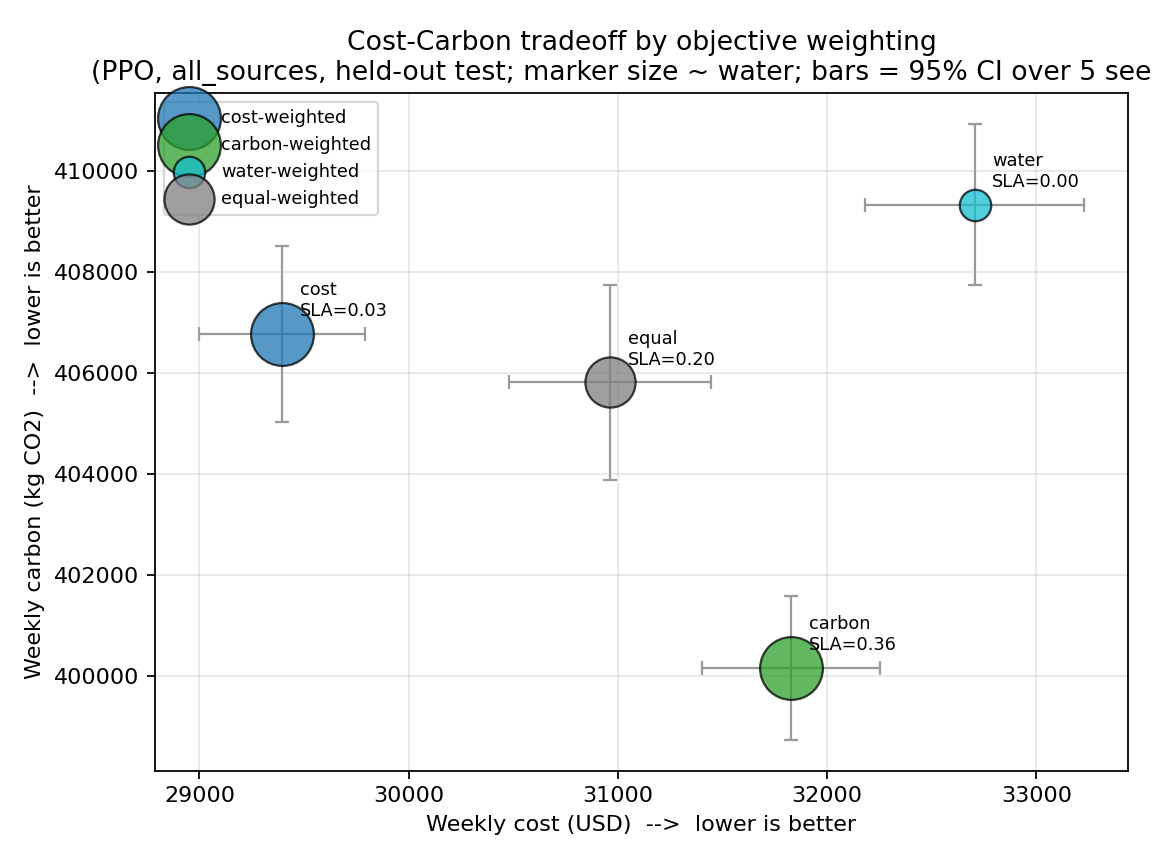
\includegraphics[keepaspectratio,alt={Figure 6}]{figures/fig_pareto_cost_carbon.png}}
\emph{Figure 6. Cost--carbon tradeoff across the four objective
weightings (marker size ∝ water; bars = 95\% CI over 20 seeds). The
weightings form a non-dominated front, but the carbon axis is compressed
--- the carbon lever is real yet small (\textasciitilde1\%) even though
grid carbon is a visible observation.}

\subsubsection{5.8 Sizing sensitivity}\label{sizing-sensitivity}

Is the large storage gap an artifact of the 20 MWh battery? We
re-evaluate RuleBased against the offline LP optimum at 10, 20, and 40
MWh (energy and power scaled together at C/2). Table IV shows the gap is
large at every size --- 14--25\% --- growing from 10→20 MWh and then
plateauing; it is not a sizing artifact and it does not shrink with more
storage.

\textbf{TABLE IV --- RuleBased→offline-optimum gap (\%) by battery
capacity, matched protocol. For contrast, the old \emph{quantile-oracle}
gap (right block) shrinks to \textasciitilde0 at 40 MWh --- the weak
oracle's artifact, not reality.}

{\def\LTcaptype{none} % do not increment counter
\begin{longtable}[]{@{}
  >{\raggedright\arraybackslash}p{(\linewidth - 10\tabcolsep) * \real{0.1429}}
  >{\raggedleft\arraybackslash}p{(\linewidth - 10\tabcolsep) * \real{0.1905}}
  >{\raggedleft\arraybackslash}p{(\linewidth - 10\tabcolsep) * \real{0.1905}}
  >{\raggedleft\arraybackslash}p{(\linewidth - 10\tabcolsep) * \real{0.1905}}
  >{\raggedright\arraybackslash}p{(\linewidth - 10\tabcolsep) * \real{0.1429}}
  >{\raggedright\arraybackslash}p{(\linewidth - 10\tabcolsep) * \real{0.1429}}@{}}
\toprule\noalign{}
\begin{minipage}[b]{\linewidth}\raggedright
Configuration
\end{minipage} & \begin{minipage}[b]{\linewidth}\raggedleft
10 MWh
\end{minipage} & \begin{minipage}[b]{\linewidth}\raggedleft
20 MWh
\end{minipage} & \begin{minipage}[b]{\linewidth}\raggedleft
40 MWh
\end{minipage} & \begin{minipage}[b]{\linewidth}\raggedright
\end{minipage} & \begin{minipage}[b]{\linewidth}\raggedright
quantile-oracle 10/20/40
\end{minipage} \\
\midrule\noalign{}
\endhead
\bottomrule\noalign{}
\endlastfoot
grid\_solar\_battery & 14.2 & 20.3 & 19.7 & & 3.9 / 4.8 / −0.0 \\
grid\_wind\_battery & 16.6 & 21.2 & 21.1 & & 4.7 / 4.4 / 0.1 \\
grid\_solar\_wind\_battery & 18.3 & 21.7 & 21.8 & & 5.6 / 4.7 / 0.9 \\
all\_sources & 22.9 & 25.1 & 24.9 & & 7.9 / 6.9 / 3.7 \\
\end{longtable}
}

Against the offline optimum the heuristic leaves \textasciitilde20--25\%
unclaimed across a fourfold sizing range, so its storage sub-optimality
is structural, not a design-point artifact. The contrast column is
itself a finding: the quantile ``oracle'' gap \emph{shrinks toward zero}
at 40 MWh --- because that threshold rule is also poor at exploiting a
large store, so it converges to RuleBased --- which is exactly how a
weak ceiling manufactures a false ``the heuristic becomes near-optimal
with more storage'' conclusion. The offline optimum shows the opposite:
more storage means more unexploited value, for both the heuristic and
(per §5.4) the learner. Training PPO on \texttt{all\_sources} at 40 MWh
confirms the learner side directly: RL loses to RuleBased by
\textbf{−6.4\%} at 40 MWh (RL \$28,071 vs RB \$26,376), a wider deficit
than the −5.0\% at 20 MWh, and it sits \textasciitilde30\% above the
offline optimum --- the RL storage shortfall widens with capacity rather
than washing out.

\pandocbounded{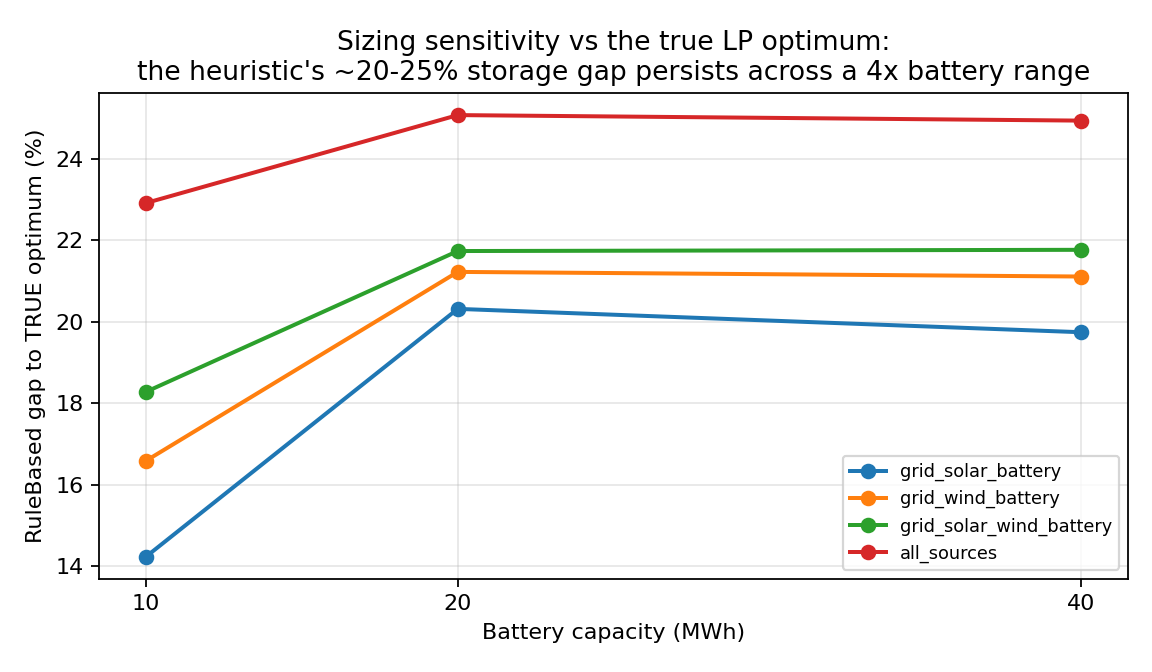
\includegraphics[keepaspectratio,alt={Figure 7}]{figures/fig_sizing_sensitivity.png}}
\emph{Figure 7. Battery-sizing sensitivity of the
RuleBased→offline-optimum gap. The \textasciitilde20--25\% storage gap
persists across a 4× sizing range (growing 10→20 MWh, then flat) ---
structural, not a sizing artifact.}

\subsubsection{5.9 Training convergence}\label{training-convergence}

Because a negative RL finding invites the objection that the learners
were simply undertrained, we log a held-out evaluation at every
100k-step checkpoint and inspect the full learning curve. Figure 8 plots
evaluation reward against training step (mean ± std over the five seeds)
for all four algorithms, on a representative renewable-only win
(\texttt{grid\_solar\_wind}) and the hardest storage loss
(\texttt{all\_sources}). Every learner \textbf{plateaus well before 1M
steps}: across the final 200k steps the mean evaluation reward changes
by less than \textbf{0.7\%} for every algorithm in both configurations
(e.g.~PPO −0.69\%, SAC +0.21\%, TD3 −0.04\%, A2C −0.58\% on
\texttt{all\_sources}). The storage-configuration losses are therefore a
\emph{converged} property of the learned policies under this training
budget, not an artifact of stopping early. A longer 2--5M-step run on
the hardest configuration is a planned confirmation (§6.6).

\pandocbounded{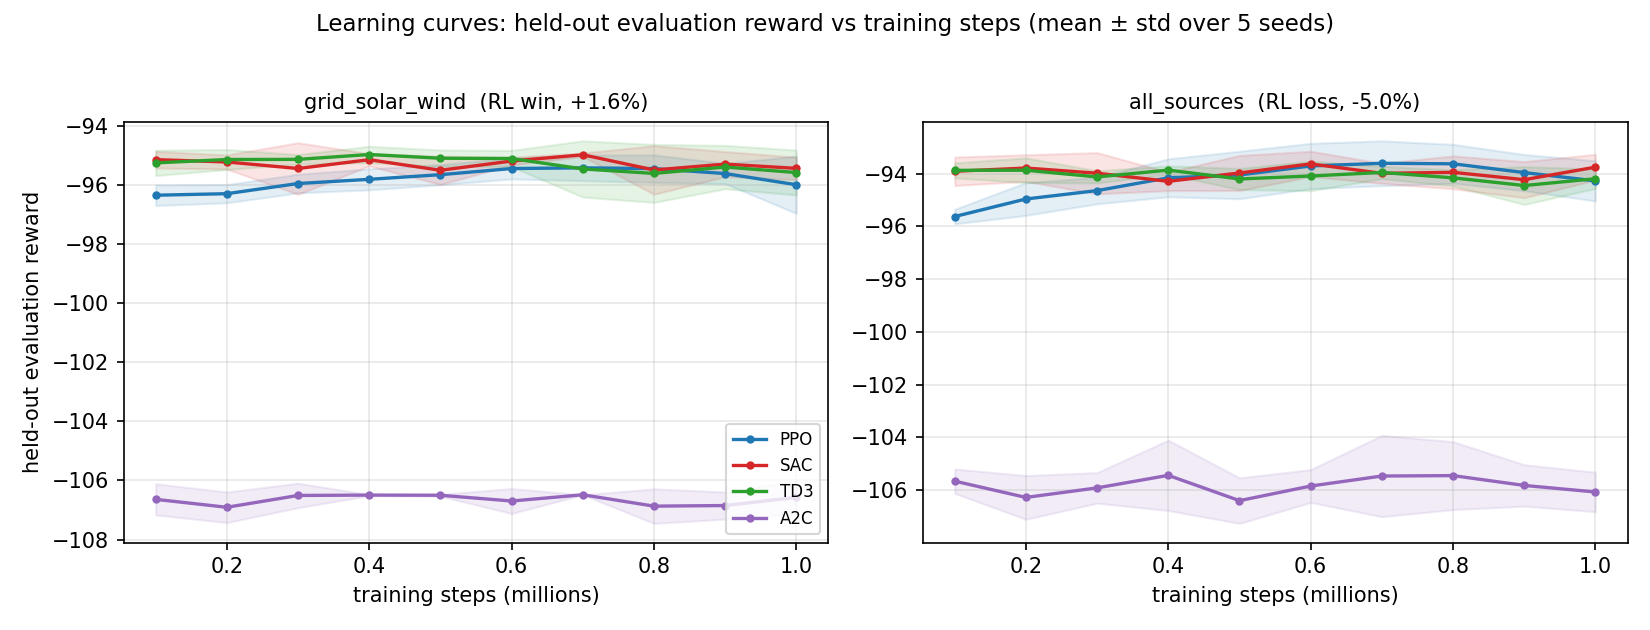
\includegraphics[keepaspectratio,alt={Figure 8}]{figures/fig_learning_curves.png}}
\emph{Figure 8. Learning curves: held-out evaluation reward vs training
steps (mean ± std over 5 seeds), for a renewable-only win (left) and the
hardest storage loss (right). All four algorithms plateau before 1M
steps; the storage losses are not an undertraining artifact.}

\begin{center}\rule{0.5\linewidth}{0.5pt}\end{center}

\subsection{6. DISCUSSION}\label{discussion}

\subsubsection{6.1 Near-optimal for renewables, far from optimal for
storage}\label{near-optimal-for-renewables-far-from-optimal-for-storage}

The heuristic's distance from the offline optimum splits cleanly by
regime, and the split is instructive. In \textbf{renewable-only}
dispatch the fixed schedule is genuinely near-optimal
(\textasciitilde6--9\% from the LP): the exploitable structure is highly
regular (ERCOT prices and solar/wind availability are strongly diurnal),
the deferral headroom is small (the replayed typical-week workload is
flat, mean ≈ 12\%, peak ≈ 15\%, so the 30\%/12 h lever moves few kWh),
and with no storage there is no inter-temporal arbitrage to get wrong
--- a time-of-use rule captures almost everything there is. Add a
\textbf{battery} and the same rule falls \textbf{20--25\% short} of the
optimum. Storage converts a near-static problem into a genuine
sequential-optimization problem: the value of charge now depends on the
entire future price/renewable path, and the optimum exploits every hour
of that path, whereas the fixed schedule commits to two windows a day
and the learner mistimes. The lesson is not ``heuristics are
near-optimal'' (the conclusion a weak quantile oracle invites) but ``the
optimality gap is small only where the problem is near-static; storage
opens a large gap that no controller we tested closes.''

\subsubsection{6.2 Why storage is where RL fails, not where it
wins}\label{why-storage-is-where-rl-fails-not-where-it-wins}

The intuitive expectation is that storage --- with its inter-temporal
coupling --- is exactly where a learner should beat a myopic rule. We
observe the opposite, and the offline optimum sharpens why. It is
\emph{not} that the fixed schedule leaves little headroom --- against
the LP it leaves 20--25\% (§5.2). Rather, storage turns each per-hour
decision into a \textbf{credit-assignment problem across the week} --- a
charge now pays off many hours later --- which is precisely where RL's
value estimates are noisiest; the off-policy learners (TD3, A2C) degrade
most, consistent with value over-/under-estimation on long-horizon
storage returns. So there is \emph{lots} of headroom, and the learner
captures even less of it than a two-window-a-day rule: RL ends up
\textbf{below} the heuristic (−1.3\% → −5.0\% as solar+wind+battery+gas
stack) while \textbf{both sit far below the optimum}. The deficit is not
a sizing artifact --- the RuleBased→optimum gap holds at 20--25\% across
a fourfold battery range (§5.8), and RL's shortfall relative to the
heuristic persists with it. In short: storage is hard for everyone here
and hardest for the learner, and the field's assumption that it is where
RL shines is exactly inverted.

\subsubsection{6.3 The economics: RL is the wrong lever, and the right
lever is
large}\label{the-economics-rl-is-the-wrong-lever-and-the-right-lever-is-large}

Two numbers should guide investment here. The first is the
RL-vs-heuristic delta: at best \textasciitilde1--1.6\% of the weekly
bill in renewable-only dispatch (\textasciitilde\$20k/yr for a
\textasciitilde10 MW site), negative everywhere a battery is present.
Against \textasciitilde\$80--120M of build capital and the cost of
training, validating, serving, and assuring a safety-critical learned
controller, a sub-2\% renewable-only trim that turns into a 1--5\%
\emph{loss} on storage does not justify RL for this problem. The second
number is the one that matters: the \textbf{20--25\% storage gap to the
offline optimum} that \emph{neither} controller captures. That is the
real, unclaimed prize, and it is an order of magnitude larger than
anything the RL-vs-heuristic contest is fighting over. The engineering
takeaway is therefore twofold: do not deploy RL for single-facility
behind-the-meter dispatch (a well-tuned heuristic is cheaper, simpler,
and better on storage), and do not conclude the problem is solved --- a
forecast-driven optimizer (§5.5) is the lever aimed at the part of the
bill that is actually on the table.

\subsubsection{6.4 Where RL adds (narrow) value: cost
steering}\label{where-rl-adds-narrow-value-cost-steering}

Where learning earns some keep is not \emph{beating} the heuristic on a
scalar objective but \textbf{steering} through the reward weights
(§5.7). A single trained policy family, re-weighted, gives an operator
predictable and statistically significant control over \textbf{cost} ---
a cost-heavy weighting is \textasciitilde5\% cheaper than a balanced one
(Welch p \textless{} 0.001) --- tracing a non-dominated front that a
fixed rule does not offer. The value is narrower than one might hope:
with 20 seeds the carbon and water levers are now statistically resolved
but \textbf{physically small} --- carbon −1.4\% (p \textless{} 0.001)
and water −1.1\% (p = 0.019) versus balanced. Crucially, this weakness
is physical, not informational: even though grid carbon is a visible
observation, the carbon lever is only \textasciitilde1\%, because
renewables are dispatched first, the battery is grid-charged, and gas is
carbon-dirty. RL here is therefore a \emph{cost-focused policy-family
generator}, not a general multi-objective knob; operators should not
expect more than marginal carbon or water control from this action
space. The small magnitude of the carbon and water levers is a caution
in itself: multi-objective authority in this setting is sensitive to
substrate fidelity and to whether the relevant signal is actually
observable to the agent.

\subsubsection{6.5 Implications for how the field
evaluates}\label{implications-for-how-the-field-evaluates}

Our results also carry a methodological message, and we are careful to
separate the two common shortcuts. \textbf{Temporal leakage} ---
sampling train and test episodes from the same record --- demonstrably
inflates the apparent advantage: in our experiments, a leaky split
reported a larger RL edge that the temporal split removed. The second
shortcut, \textbf{oracle price foresight} in the observation, we tested
head-on (§5.6) and found it does \emph{not} help the learned controller
here (mean premium ≈0); so in our case its removal is not what drives
the verdict, but it remains bad practice because it flatters
forecast-driven controllers and is undeployable. The honest picture is
thus doubly robust: the advantage is small under a leakage-free split,
and it does not grow even with perfect foresight. Because these
shortcuts are widespread, some reported single-site RL gains are
plausibly evaluation artifacts rather than control skill. We therefore
argue that leakage-free splits, oracle-free observations, and a
\emph{well-tuned heuristic reported as the comparator} (not a strawman)
should be the default hygiene for this literature.

\subsubsection{6.6 Scope and where learning should
help}\label{scope-and-where-learning-should-help}

These conclusions are bounded by the reliable-grid, cost-smooth regime
studied here (§7). The natural place to expect a genuine RL advantage is
where the environment is \textbf{non-stationary and event-driven} rather
than smoothly diurnal --- most sharply, on \textbf{unreliable grids}
where unscheduled outages make outage-aware on-site dispatch and diesel
avoidance a high-variance, high-stakes control problem in which a fixed
schedule cannot anticipate the disruption. That regime, using real
outage data, is the subject of a companion study; the honest, reusable
benchmark established here is its foundation. A recent critical review
of energy-storage solutions for AI data centers (Mohammadi et al.~2026,
arXiv:2603.00415) independently identifies gaps in simulation tools,
degradation and forecasting models, and multi-layer sizing as open
challenges --- the same integration gap this benchmark is built to
probe.

Several planned robustness checks would further stress-test the
conclusions and are the natural extensions of this benchmark: (i) a
longer 2--5M-step training run on the hardest storage configuration, to
confirm the plateau of §5.9 at a larger budget; (ii) injecting
stochasticity into the replayed workload and testing a second trace, to
rule out the deterministic-load explanation (§7.13); (iii) a
\textbf{realistic-forecast} MPC (finite forecast error) to measure how
much of the perfect-foresight LP gap a competent online optimizer can
actually close; (iv) a fully agent-controlled battery (no automatic
renewable charging) to isolate the effect of that dynamic; (v) a battery
round-trip-efficiency sweep (0.85 / 0.90 / 0.95); (vi) a
hyperparameter-robustness sweep for PPO and SAC; and --- most important
--- (vii) \textbf{recurrent policies (LSTM/Transformer)}, the natural
architecture for the long-horizon storage credit-assignment problem that
our feedforward learners handle worst (§4.3, §6.2): whether memory
closes the storage gap is the sharpest open question this benchmark
poses. Each targets a specific alternative explanation rather than the
headline finding, which the leakage-free protocol, the foresight
ablation, and the convergence curves already support for the feedforward
policies studied here.

\begin{center}\rule{0.5\linewidth}{0.5pt}\end{center}

\subsection{7. THREATS TO VALIDITY}\label{threats-to-validity}

\begin{enumerate}
\def\labelenumi{\arabic{enumi}.}
\item
  \textbf{Sub-hour burst smoothing.} The trace provides per-instance
  lifetime-average usage, so the reconstructed load smooths sub-hourly
  bursts; standard for this trace and disclosed.
\item
  \textbf{GPU-dominated, heterogeneous facility.} The trace is a GPU
  cluster; utilization→power is GPU-TDP-based. We frame the facility as
  an AI data center accordingly.
\item
  \textbf{Replayed, not calendar-real, load.} Trace timestamps are
  desensitized; the load is real in structure but not a real calendar
  sequence, and the temporal split is applied to the grid signals where
  leakage actually lives.
\item
  \textbf{Modeled power and cooling.} The load is real, but IT power and
  cooling are models, not metered facility telemetry. The comparative
  conclusions are therefore more robust than any single absolute figure.
\item
  \textbf{Single facility, modeled sizing.} Mitigated by the sizing
  sensitivity of §5.8, which shows the central result is stable across a
  4× battery range.
\item
  \textbf{ERCOT-only multi-year run.} CAISO history begins in 2023;
  cross-market generalization is future work.
\item
  \textbf{Simulation, not deployment.} Standard in this field
  (Green-DCC, Sustain-Cluster are also simulation studies).
\item
  \textbf{Modeled substrate parameters.} The substrate depends on
  several modeled constants (Table VI). The key robustness argument is
  structural: because \emph{every} controller --- RL, heuristics, and
  the oracle --- is evaluated on the \emph{same} substrate, changing
  these parameters shifts the \emph{absolute} cost/carbon/water levels
  but largely preserves the \emph{relative} comparisons the paper
  reports. In particular, the \textbf{sign of the RL-vs-heuristic
  difference} (RL loses on storage) and the \textbf{ordering of the
  online-to-offline gap} (small for renewables, large for storage) are
  properties of the dispatch structure, not of the exact parameter
  values, because every controller --- RL, heuristics, and the LP
  optimum --- is scored on the same substrate and seeds. Parameters that
  enter only one objective (e.g.~the water coefficient) move that
  objective's absolute level without touching the cost verdict. We
  regard the exact magnitude of the storage gap (20--25\%) as
  parameter-dependent at the ±few-point level, but its existence and the
  qualitative renewable-vs-storage split as robust.

  \textbf{TABLE VI --- Modeled parameters and sensitivity scope.}

  {\def\LTcaptype{none} % do not increment counter
  \begin{longtable}[]{@{}
    >{\raggedright\arraybackslash}p{(\linewidth - 8\tabcolsep) * \real{0.2000}}
    >{\raggedright\arraybackslash}p{(\linewidth - 8\tabcolsep) * \real{0.2000}}
    >{\raggedright\arraybackslash}p{(\linewidth - 8\tabcolsep) * \real{0.2000}}
    >{\raggedright\arraybackslash}p{(\linewidth - 8\tabcolsep) * \real{0.2000}}
    >{\raggedright\arraybackslash}p{(\linewidth - 8\tabcolsep) * \real{0.2000}}@{}}
  \toprule\noalign{}
  \begin{minipage}[b]{\linewidth}\raggedright
  Parameter
  \end{minipage} & \begin{minipage}[b]{\linewidth}\raggedright
  Baseline
  \end{minipage} & \begin{minipage}[b]{\linewidth}\raggedright
  Plausible range
  \end{minipage} & \begin{minipage}[b]{\linewidth}\raggedright
  Primarily affects
  \end{minipage} & \begin{minipage}[b]{\linewidth}\raggedright
  Expected effect on the verdict
  \end{minipage} \\
  \midrule\noalign{}
  \endhead
  \bottomrule\noalign{}
  \endlastfoot
  Idle fraction φ & 0.30 & 0.20--0.40 & facility load / absolute cost &
  shifts levels; relative verdict robust \\
  PUE\_min & 1.25 & 1.10--1.40 & cooling share / cost & shifts levels;
  relative verdict robust \\
  PUE slope s & 0.01 /°C & 0.005--0.02 & cooling vs temperature & minor;
  relative verdict robust \\
  Solar eff.×PR & 0.18 × 0.85 & ±20\% & renewable availability & may
  slightly change renewable-config margins \\
  Wind cut-in / rated & 3.5 / 12 m/s & ±1 / ±2 m/s & wind availability &
  may slightly change wind-config margins \\
  Gas emission factor & 0.41 kgCO₂/kWh & 0.35--0.55 & carbon in gas
  configs & affects carbon objective, not cost verdict \\
  Water coefficient & 1.8 & ±25\% & water objective only & isolated to
  water; no cost effect \\
  IT-power envelope & linear (Fan) & SPEC-power convex alt. & IT power
  shape & shifts levels; relative verdict robust \\
  \end{longtable}
  }

  8a. \textbf{The LP optimum is a conservative ceiling.} The LP does not
  exploit the cooling-offset cost lever and models deferral with the
  environment's own 1/12-per-hour backlog drain rather than free
  load-shifting; both make it \emph{under}-optimize slightly, so the
  reported optimality gaps (20--25\% on storage) are \textbf{lower
  bounds} on the true gap. It is verified to satisfy LP ≤ RuleBased on
  every episode.
\item
  \textbf{MPC ran on a persistence forecast.} Disclosed; ours is a
  naive-forecast MPC included only to show a zero-information forecast
  buys nothing. Per §5.5 the LP optimum (a perfect-foresight optimizer)
  captures the 20--25\% storage headroom, so a competent forecast-driven
  MPC is the natural next controller and a promising route to close the
  gap --- future work.
\item
  \textbf{Reward-normalization divisors use full-record statistics.} The
  data-derived divisors C, K, W (§3.7) are the mean hourly
  cost/carbon/water over the entire 2020--2025 record, including the
  2024--2025 test window. This is a mild normalization dependency, not
  an outcome leak: the divisors are fixed scalars that only \emph{shape
  the training reward}; every \textbf{reported} cost/carbon/water figure
  is an absolute physical quantity computed independently of them, and
  all controllers are scored identically. Recomputing the divisors on
  the training window only would not affect the reported numbers. For
  scale, the train-only cost divisor would be ≈733 versus the 592 used
  (a 19\% difference, because the 2024--25 test window is a cheaper
  price regime than the 2020--23 training window) --- a reward-shaping
  offset identical across all controllers, not an evaluation leak.
\item
  \textbf{Implicit environment dynamics around storage.} Two dispatch
  behaviors are deterministic properties of the substrate rather than
  agent choices, and we disclose them because they shape the storage
  results: (a) surplus on-site renewable auto-charges the battery up to
  95\% SoC \emph{regardless of the agent's battery action} (§3.4), so
  SoC is not fully controllable from the explicit action; and (b) the
  SLA penalty \emph{latches} --- once any violation occurs it is charged
  every remaining hour of the episode (§3.7). Both are identical across
  all controllers, so they do not bias the relative comparison, but they
  help explain why storage coordination is hard for the learner (§6.2).
  We note that the auto-charging reduces the agent's \emph{control
  authority} over one state dimension but does \textbf{not} violate the
  Markov property: the observation includes SoC, current renewable
  availability, and current demand, so the SoC transition is a
  deterministic function of the observed state and action --- even
  though the agent's battery action alone does not uniquely determine
  it.
\item
  \textbf{Foresight-ablation seed parity.} The foresight premium (§5.6)
  pairs the oracle-mode and persistence-mode PPO runs by construction
  --- both were launched from the same
  \texttt{EVAL\_SEED\_BASE\ =\ 8000} held-out seed set (8000--8199) in
  the same harness --- but this parity is assumed from the launch
  configuration rather than re-verified episode-by-episode from a stored
  seed vector in each artifact. A per-episode seed-hash check is left as
  a hardening item.
\item
  \textbf{Deterministic replayed load.} The workload is a fixed
  typical-week profile replayed across the horizon (§3.2), so load is
  deterministic while price, weather, and carbon vary. This removes one
  source of stochasticity and could, in principle, narrow the advantage
  a learner might extract from adapting to load fluctuations. Two points
  bound the concern: the structure the controllers actually compete over
  --- diurnal price/renewable variation and multi-hour storage arbitrage
  --- is present independent of load stochasticity, and the storage
  credit-assignment difficulty (§6.2) does not arise from load noise.
  Injecting load variability (and testing a second workload trace) is a
  planned robustness check (§6).
\item
  \textbf{Training convergence.} A negative RL result invites an
  undertraining objection. Figure 8 (§5.9) shows all four algorithms
  plateau well before 1M steps --- held-out reward changes by
  \textless0.7\% over the final 200k steps on both a renewable-only win
  and the hardest storage loss --- so the storage losses are a converged
  property of the learned policies. A longer 2--5M-step run on the
  hardest configuration is a planned confirmation (§6).
\item
  \textbf{Asymmetric search difficulty.} The RL controllers optimize a
  4-dimensional continuous action space (deferral, cooling, battery,
  gas) online, whereas RuleBased is a near-deterministic fixed schedule;
  the learner is therefore solving a substantially larger search
  problem. This is inherent to comparing a learned controller against a
  fixed rule and does not affect the cost comparison itself --- both are
  scored on identical held-out weeks --- but it is part of why a simple
  rule is a demanding baseline, and it reinforces the practical point
  (§6.3) that the added search and assurance burden of RL is not repaid
  here.
\end{enumerate}

\begin{center}\rule{0.5\linewidth}{0.5pt}\end{center}

\subsection{8. CONCLUSION}\label{conclusion}

On an honest, leakage-free, real-trace benchmark for single-facility
behind-the-meter dispatch, deep reinforcement learning beats a
well-tuned time-of-use heuristic in only \textbf{4 of 12} configurations
--- all renewable-only, by 0.5--1.6\% --- and significantly
\emph{underperforms} it in every storage configuration, to −5.0\% at the
full asset mix; handing the learner perfect price foresight changes
essentially nothing for either PPO or SAC. So the field's premise is at
best half-right: sophistication is not free, and a well-tuned heuristic
is a strong baseline that learning here rarely beats and often loses to
--- at least for the feedforward policies evaluated here; whether
recurrent architectures change the storage verdict is the key open
question we leave to future work (§6.6).

But the more consequential finding comes from measuring against a
\emph{true} per-episode LP optimum rather than the quantile-threshold
``oracle'' this literature usually reports. That correction alone flips
the standard conclusion: the heuristic is near-optimal
(\textasciitilde6--9\%) only in renewable-only dispatch, while in
storage-rich configurations \textbf{both the heuristic and RL sit
\textasciitilde20--25\% above the offline optimum} --- a large
online-to-offline gap that persists across a fourfold battery range and
that no controller we tested closes. Perfect foresight is worth that
20--25\% to the optimum yet \textasciitilde0\% to the learners, which
locates the bottleneck precisely: online storage coordination under
uncertainty, not forecast quality or the choice between heuristic and
RL. RL's one usable affordance is cost-weighted steering
(\textasciitilde5\%); its carbon and water levers, though now
statistically resolved, are physically small (\textasciitilde1\%).

The practical verdict is therefore that RL is the wrong lever for this
problem, but the problem is far from solved: the prize is the storage
gap, and a forecast-driven optimizer is the controller aimed at it.
Methodologically, we argue that leakage-free splits, oracle-free
observations, a well-tuned heuristic reported as the comparator,
\textbf{and a genuine optimization-based ceiling} should be the default
hygiene for this literature --- because a weak ``oracle'' manufactures a
comfortable ``heuristics are near-optimal'' story that a real optimum
does not support. The honest, reusable benchmark established here is the
foundation for the harder, non-stationary regime --- unreliable grids
with real outages --- where a fixed schedule cannot anticipate the
disruption and learned control may finally earn its keep (a companion
study).

\begin{center}\rule{0.5\linewidth}{0.5pt}\end{center}

\subsection{9. REPRODUCIBILITY}\label{reproducibility}

\textbf{Artifacts.} All code and result artifacts are released in a
public repository
(https://github.com/dev1-osibo/neither-near-optimal-nor-learnable): the
simulation environment, the baseline controllers, the offline-optimum LP
solver, the training harness, the evaluation and analysis scripts, the
automated integrity tests, the fixed seeds, and the exact temporal
split, together with a data-provenance description and the full set of
result files. Every table and figure in this paper regenerates from the
released artifacts with a single command, and the complete parameter set
is consolidated in Table V.

\textbf{Automated integrity checks.} The two claims the paper leans on
hardest are backed by unit tests rather than assertion. (i) \emph{No
forecast leakage:} \texttt{tests/test\_env\_forecast\_leakage.py}
corrupts every price after time \emph{t} by a large spike and verifies
the two forecast observation dimensions at \emph{t} are unchanged in the
reported \texttt{persistence} mode; a companion test confirms
\texttt{oracle} mode \emph{does} react to future prices (so the test can
actually detect leakage), and a third asserts the default constructor is
the honest \texttt{persistence} mode. (ii) \emph{Correct workload
reconstruction:} \texttt{tests/test\_workload\_trace.py} checks the
hourly utilization equals active usage divided by machine capacity on a
known toy cluster, that utilization is bounded to {[}0, 1{]} even under
excessive usage, and that the fitted typical-week model preserves
diurnal structure (peak-hour mean \textgreater{} trough-hour mean) when
replayed.

\textbf{Determinism / provenance note.} The full campaign comprises 445
runs (240 main + 120 foresight {[}PPO+SAC{]} + 80 Pareto {[}20 seeds{]}
+ 5 sizing), with zero failures, executed across two matched-environment
machines; a byte-identical data-and-code check confirmed both used one
canonical substrate, and fixed seeds make every run reproducible.

\textbf{Licensing.} The workload trace is used under the Alibaba Cluster
Trace Program research license (Weng et al.~2022); market (ERCOT),
carbon (EIA + IPCC), and weather (Open-Meteo / NASA POWER) sources are
cited in §3.4.

\begin{center}\rule{0.5\linewidth}{0.5pt}\end{center}

\subsection{REFERENCES}\label{references}

\emph{Formatted in ASA (American Sociological Association) style;
in-text citations are author--date, e.g., (Weng et al.~2022).
Web-verified bibliography with locators is maintained in
\texttt{paper/REFERENCES.md}.}

Abdelhady, Mohamed Hamdi Ibrahim, Eleftherios T. Iakovou, and Efstratios
N. Pistikopoulos. 2026. ``Optimal Energy Portfolio Investment Strategies
for Data Centers under Deep Market Uncertainty.'' \emph{Applied Energy}.

Electric Power Research Institute. 2024. ``DCFlex: Data Center Flexible
Load Initiative.'' Palo Alto, CA: EPRI. Retrieved
(https://www.epri.com).

Fan, Xiaobo, Wolf-Dietrich Weber, and Luiz André Barroso. 2007. ``Power
Provisioning for a Warehouse-Sized Computer.'' Pp. 13--23 in
\emph{Proceedings of the 34th Annual International Symposium on Computer
Architecture}. New York: ACM.

Figini, Enea, and Mario Paolone. 2025. ``Achieving Dispatchability in
Data Centers: Carbon and Cost-Aware Sizing of Energy Storage and Local
Photovoltaic Generation.'' \emph{Sustainable Energy, Grids and Networks}
43:101920. doi:10.1016/j.segan.2025.101920. arXiv:2412.13853.

Fujimoto, Scott, Herke van Hoof, and David Meger. 2018. ``Addressing
Function Approximation Error in Actor-Critic Methods.'' Presented at the
35th International Conference on Machine Learning (ICML), Stockholm,
Sweden. arXiv:1802.09477.

Guillen-Perez, Antonio, Avisek Naug, Vineet Gundecha, Sahand
Ghorbanpour, Ricardo Luna Gutierrez, Ashwin Ramesh Babu, Munther Salim,
Shubhanker Banerjee, Eoin H. Oude Essink, Damien Fay, and Soumyendu
Sarkar. 2025. ``DCcluster-Opt: Benchmarking Dynamic Multi-Objective
Optimization for Geo-Distributed Data Center Workloads.'' Presented at
the Conference on Neural Information Processing Systems (NeurIPS),
Datasets and Benchmarks Track. arXiv:2511.00117.

Haarnoja, Tuomas, Aurick Zhou, Pieter Abbeel, and Sergey Levine. 2018.
``Soft Actor-Critic: Off-Policy Maximum Entropy Deep Reinforcement
Learning with a Stochastic Actor.'' Presented at the 35th International
Conference on Machine Learning (ICML), Stockholm, Sweden.
arXiv:1801.01290.

International Energy Agency. 2025. \emph{Energy and AI}. Paris:
International Energy Agency. Retrieved
(https://www.iea.org/reports/energy-and-ai).

Iqbal, Hasan, and Arif I. Sarwat. 2026. ``Reliability-Constrained
Behind-the-Meter BESS Dispatch for Data Centers: Co-Optimizing Utility
Costs and Critical-Load Continuity Under Stochastic Outages.''
\emph{IEEE Access} 14:79227--79252.

Lazic, Nevena, Craig Boutilier, Tyler Lu, Eehern Wong, Binz Roy,
Moonkyung Ryu, and Greg Imwalle. 2018. ``Data Center Cooling Using
Model-Predictive Control.'' In \emph{Advances in Neural Information
Processing Systems 31 (NeurIPS)}.

Lim, Bryan, Sercan Ö. Arık, Nicolas Loeff, and Tomas Pfister. 2021.
``Temporal Fusion Transformers for Interpretable Multi-Horizon Time
Series Forecasting.'' \emph{International Journal of Forecasting}
37(4):1748--1764.

Liu, Shaohui, Sungho Shin, and Deepjyoti Deka. 2026. ``Watts vs.~Bytes:
Turning Data Centers into Grid Assets via Storage--Compute
Co-Optimization.'' arXiv:2605.16190.

Mnih, Volodymyr, Adrià P. Badia, Mehdi Mirza, Alex Graves, Timothy P.
Lillicrap, Tim Harley, David Silver, and Koray Kavukcuoglu. 2016.
``Asynchronous Methods for Deep Reinforcement Learning.'' Pp. 1928--1937
in \emph{Proceedings of the 33rd International Conference on Machine
Learning (ICML)}. arXiv:1602.01783.

Mohammadi, Sina, Wayne Wang, Marcus Chen-I Wada, Rouzbeh Haghighi, Ali
Hassan, Hualong Liu, Archit Bhatnagar, Ang Chen, and Wencong Su. 2026.
``Grid Integration of AI Data Centers: A Critical Review of Energy
Storage Solutions.'' arXiv:2603.00415.

Naug, Avisek, Antonio Guillen, Ricardo Luna Gutierrez, Vineet Gundecha,
Sahand Ghorbanpour, Sajad Mousavi, Ashwin Ramesh Babu, and Soumyendu
Sarkar. 2024. ``SustainDC: Benchmarking for Sustainable Data Center
Control.'' Presented at the Conference on Neural Information Processing
Systems (NeurIPS), Datasets and Benchmarks Track. arXiv:2408.07841.

Osibo, Babasola. 2025. ``Transforming High-Energy Data Center Sites:
Sustainability with Predictive Analytics and Futuristic Technologies.''
\emph{International Journal of Science and Research} 14(8):903--911.
doi:10.21275/SR25816234249.

Osibo, Babasola, and Simisola Adamo. 2023. ``Data Centers and Green
Energy: Paving the Way for a Sustainable Digital Future.''
\emph{International Journal of Latest Technology in Engineering,
Management \& Applied Science} 12(11):15--30.
doi:10.51583/IJLTEMAS.2023.121103.

Radovanović, Ana, Ross Koningstein, Ian Schneider, Bokan Chen, Alexandre
Duarte, Binz Roy, Diyue Xiao, Maya Haridasan, Patrick Hung, Nick Care,
Saurav Talukdar, Eric Mullen, Kendal Smith, MariEllen Cottman, and
Walfredo Cirne. 2023. ``Carbon-Aware Computing for Datacenters.''
\emph{IEEE Transactions on Power Systems} 38(2), March.
arXiv:2106.11750.

Raffin, Antonin, Ashley Hill, Adam Gleave, Anssi Kanervisto, Maximilian
Ernestus, and Noah Dormann. 2021. ``Stable-Baselines3: Reliable
Reinforcement Learning Implementations.'' \emph{Journal of Machine
Learning Research} 22(268):1--8.

Rafique, Abubakar, Xiaojun Yu, Muhammad Jawad, Qun Song, Zhaohui Yuan,
Muhammad Tariq Sadiq, Kamran Daniel, and Noman Shabbir. 2026.
``Two-Stage Optimization-Learning Framework for Uncertainty-Aware
Multi-Zonal Data Center Energy Management.'' \emph{Energies} 19(7):1736.
doi:10.3390/en19071736.

Sarkar, Soumyendu, Avisek Naug, Antonio Guillen, Vineet Gundecha,
Ricardo Luna Gutierrez, Sahand Ghorbanpour, Sajad Mousavi, Ashwin Ramesh
Babu, Desik Rengarajan, and Cullen Bash. 2025. ``Hierarchical
Multi-Agent Framework for Carbon-Efficient Liquid-Cooled Data Center
Clusters (Green-DCC).'' arXiv:2502.08337.

Schulman, John, Filip Wolski, Prafulla Dhariwal, Alec Radford, and Oleg
Klimov. 2017. ``Proximal Policy Optimization Algorithms.''
arXiv:1707.06347.

U.S. Energy Information Administration. 2024. ``Hourly Electric Grid
Monitor'' (fuel mix by balancing authority). Washington, DC: EIA.
Retrieved (https://www.eia.gov).

Waltz, Emily, and Dina Genkina. 2026. ``Small Data Centers Snuggle Up to
Grid Substations.'' \emph{IEEE Spectrum}, July. Retrieved
(https://spectrum.ieee.org/distributed-inference-data-centers).

Weng, Qizhen, Wencong Xiao, Yinghao Yu, Wei Wang, Cheng Wang, Jian He,
Yong Li, Liping Zhang, Wei Lin, and Yu Ding. 2022. ``MLaaS in the Wild:
Workload Analysis and Scheduling in Large-Scale Heterogeneous GPU
Clusters.'' In \emph{Proceedings of the 19th USENIX Symposium on
Networked Systems Design and Implementation (NSDI)}. Berkeley, CA:
USENIX Association.

\emph{Additional data sources (Data Availability, §3.4/§9): ERCOT market
LMPs; IPCC emission factors; ASHRAE TC 9.9 thermal guidelines;
Open-Meteo and NASA POWER weather. A few conference page ranges (Weng et
al.; Lazic et al.) are omitted where USENIX/NeurIPS proceedings do not
paginate; arXiv identifiers and DOIs are provided as stable locators.}

\end{document}
